\documentclass{book}
\usepackage[letterpaper,top=2.5cm,bottom=2.5cm,left=2.5cm,right=2.5cm]{geometry}
\usepackage{makeidx}
\usepackage{natbib}
\usepackage{graphicx}
\usepackage{multicol}
\usepackage{float}
\usepackage{listings}
\usepackage{color}
\usepackage{ifthen}
\usepackage[table]{xcolor}
\usepackage{textcomp}
\usepackage{alltt}
\usepackage{ifpdf}
\ifpdf
\usepackage[pdftex,
            pagebackref=true,
            colorlinks=true,
            linkcolor=blue,
            unicode
           ]{hyperref}
\else
\usepackage[ps2pdf,
            pagebackref=true,
            colorlinks=true,
            linkcolor=blue,
            unicode
           ]{hyperref}
\usepackage{pspicture}
\fi
\usepackage[utf8]{inputenc}
\usepackage{mathptmx}
\usepackage[scaled=.90]{helvet}
\usepackage{courier}
\usepackage{sectsty}
\usepackage{amssymb}
\usepackage[titles]{tocloft}
\usepackage{doxygen}
\lstset{language=C++,inputencoding=utf8,basicstyle=\footnotesize,breaklines=true,breakatwhitespace=true,tabsize=4,numbers=left }
\makeindex
\setcounter{tocdepth}{3}
\renewcommand{\footrulewidth}{0.4pt}
\renewcommand{\familydefault}{\sfdefault}
\hfuzz=15pt
\setlength{\emergencystretch}{15pt}
\hbadness=750
\tolerance=750
\begin{document}
\hypersetup{pageanchor=false,citecolor=blue}
\begin{titlepage}
\vspace*{7cm}
\begin{center}
{\Large ez\-L\-C\-D Python Module \\[1ex]\large 1.\-02 }\\
\vspace*{1cm}
{\large Generated by Doxygen 1.8.3.1}\\
\vspace*{0.5cm}
{\small Fri Jul 19 2013 15:21:39}\\
\end{center}
\end{titlepage}
\clearemptydoublepage
\pagenumbering{roman}
\tableofcontents
\clearemptydoublepage
\pagenumbering{arabic}
\hypersetup{pageanchor=true,citecolor=blue}
\chapter{Main Page}
\label{index}\hypertarget{index}{}  
\begin{DoxyImageNoCaption}
  \mbox{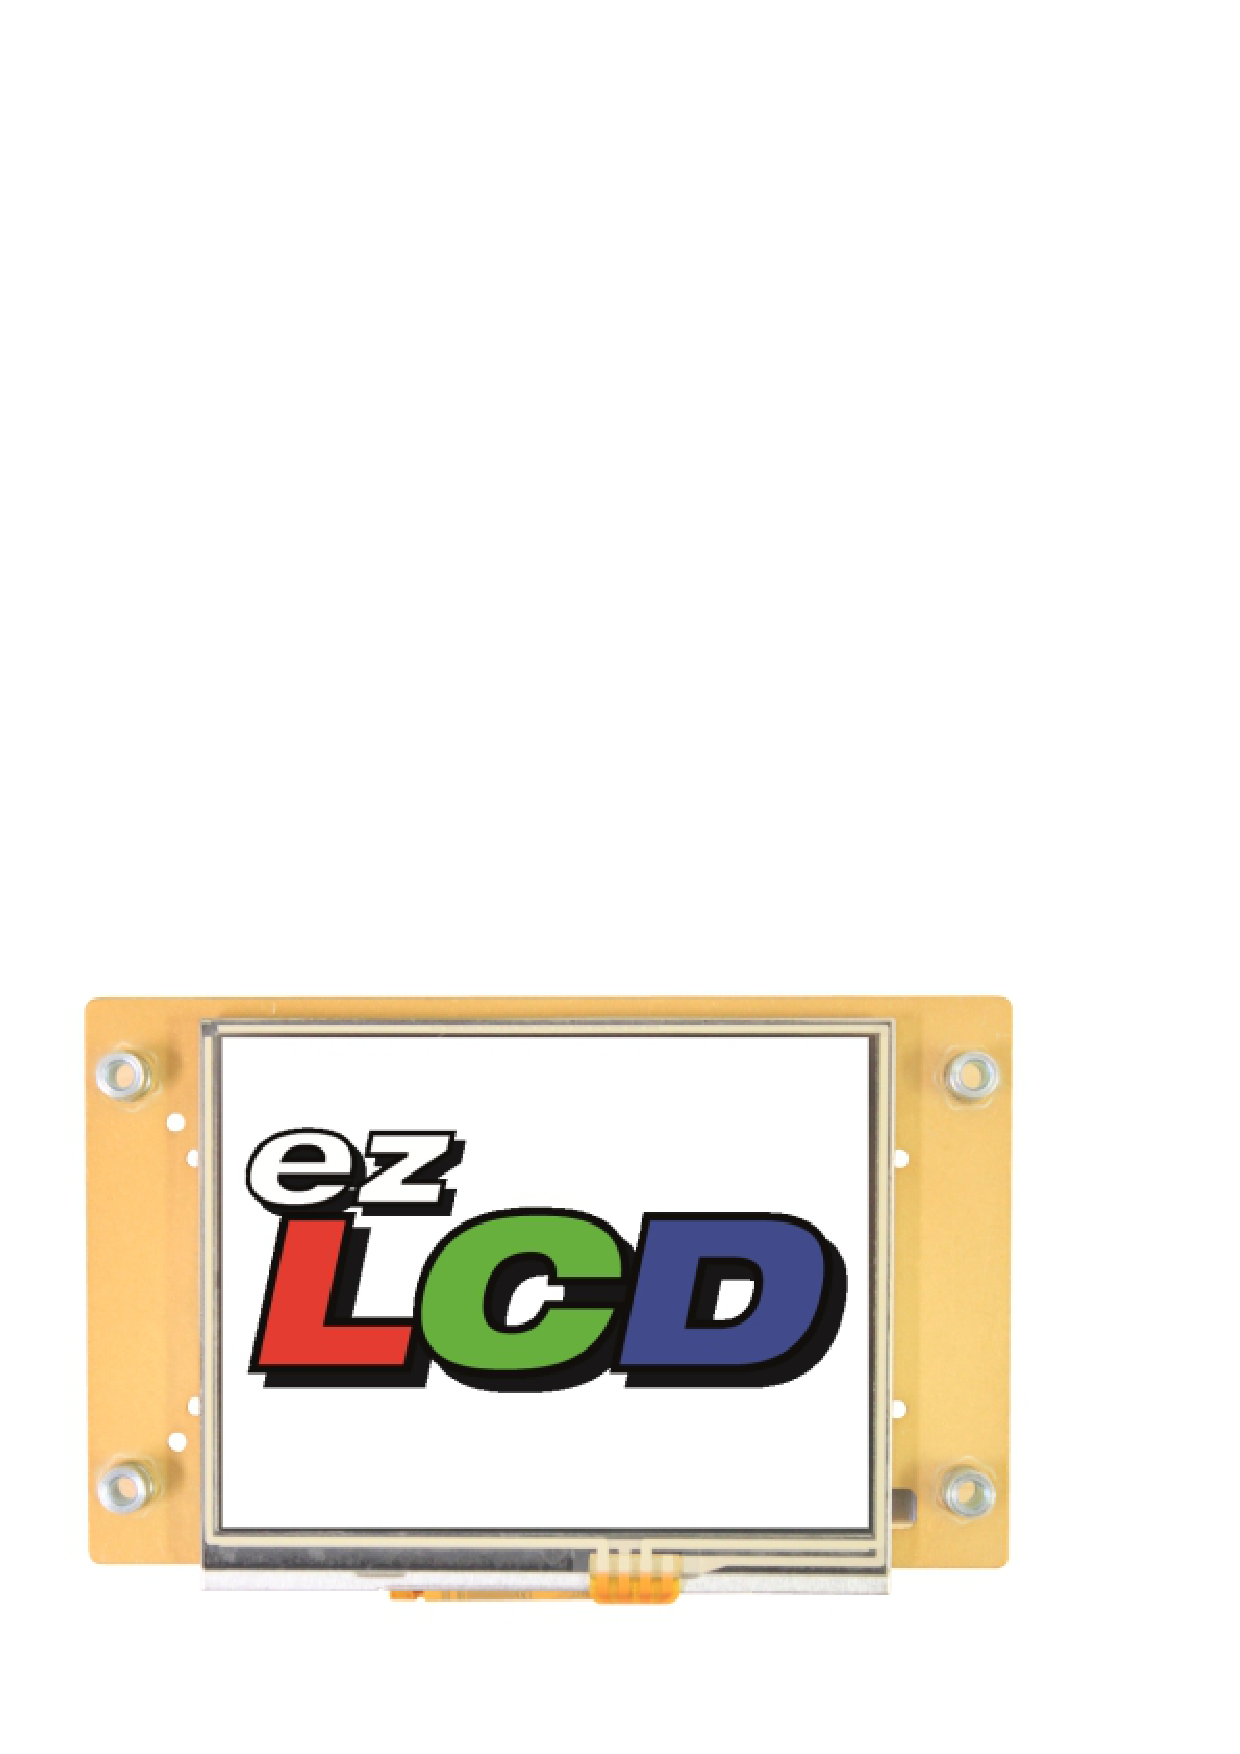
\includegraphics{ezLCD-303Front.png}}
\end{DoxyImageNoCaption}
 
\begin{DoxyImageNoCaption}
  \mbox{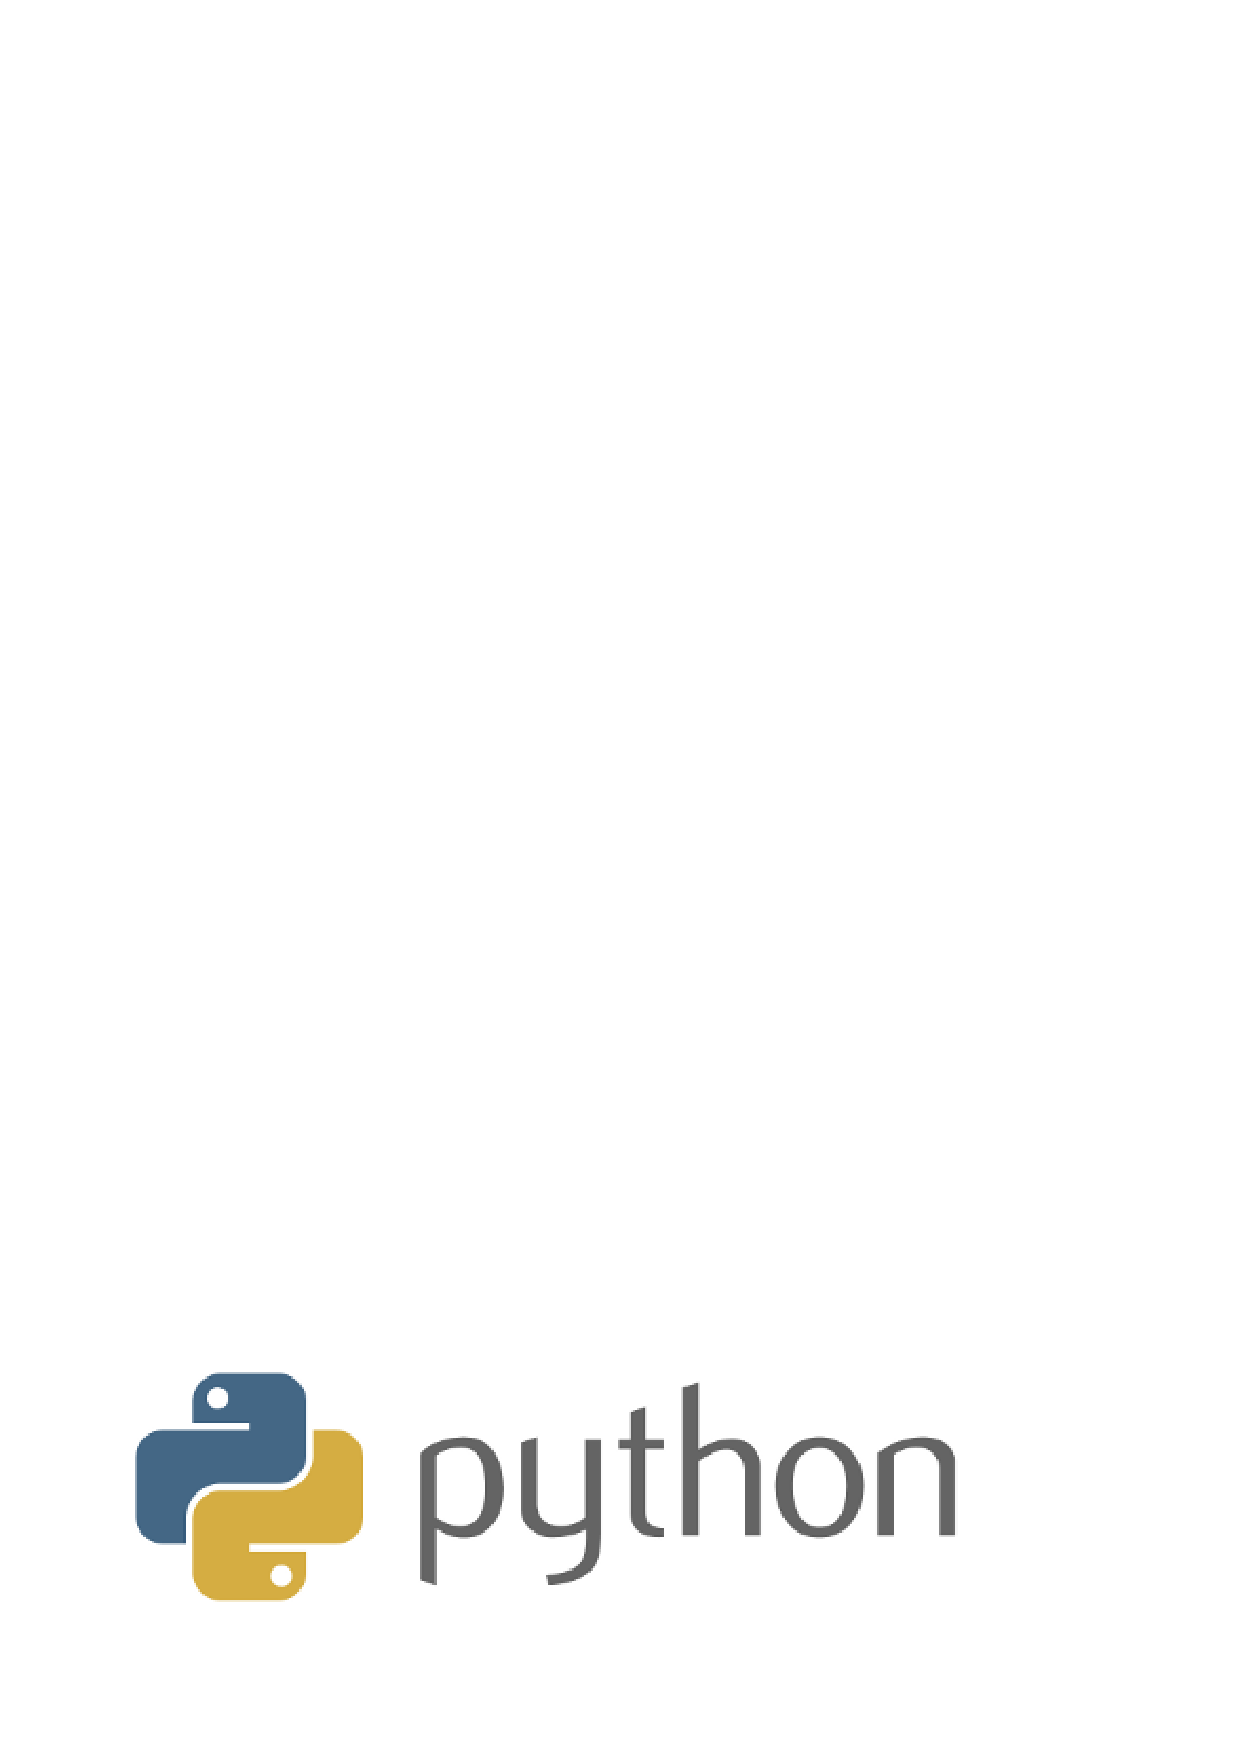
\includegraphics{python.png}}
\end{DoxyImageNoCaption}
 
\chapter{Introduction To The Hardware}
\label{introHardware}
\hypertarget{introHardware}{}
The ez\-L\-C\-D modules comtains a G\-P\-U an related circutry to drive a L\-C\-D display, U\-S\-B interface \par
 Internal 4mb M\-S\-D flash drive for storage of fonts, bitmaps and macros.\par
 Display can be controlled through U\-S\-B C\-D\-C Serial or T\-T\-L 3.\-3v Serial .\par
 \par
 Commands are sent to the ez\-L\-C\-D though the serial interface, Commands are text based and end with a carrage return {\bfseries cr}.\par
 So if you send {\bfseries cls} ending with a {\bfseries cr} the device will clear the screen and return a {\bfseries cr} when the command is complete,\par
 some widgets take a bit of time (in the millsecond range) to complete so after sending a command allways wait for a {\bfseries cr} to comeback before sending another command.\par

\chapter{Introduction To The Software}
\label{introSoftware}
\hypertarget{introSoftware}{}
Minimal example will open the ez\-L\-C\-D port clear the screen and print 'Hello From Python' in red \par
  
\begin{DoxyCodeInclude}
1 \textcolor{comment}{# Minimal ezLCD Python demo}
2 \textcolor{comment}{#}
3 
4 \textcolor{keyword}{import} platform
5 \textcolor{keyword}{import} sys
6 
7 
8 sys.path.append(\textcolor{stringliteral}{"C:\(\backslash\)Users\(\backslash\)codeman\(\backslash\)Documents\(\backslash\)GitHub\(\backslash\)ezLCD3xxPython\(\backslash\)module"}) 
9 \textcolor{keyword}{from} ezLCD3xx \textcolor{keyword}{import} *
10 
11 \textcolor{comment}{#check what OS we are on}
12 \textcolor{comment}{#Windows}
13 \textcolor{keywordflow}{if} platform.system() == \textcolor{stringliteral}{'Windows'}:
14     LCD = ezLCD(\textcolor{stringliteral}{'com6'}) 
15 \textcolor{comment}{#Mac}
16 \textcolor{keywordflow}{elif} platform.system() == \textcolor{stringliteral}{'Dawrwin'}:
17     LCD = ezLCD(\textcolor{stringliteral}{'/dev/tty.usbsomething'})
18 \textcolor{comment}{# Bail out if comport error}
19 \textcolor{keywordflow}{if} LCD.openSerial()==\textcolor{keyword}{False}:
20     \textcolor{keywordflow}{print} \textcolor{stringliteral}{'Error Opening Port'}
21     \textcolor{keywordflow}{raise} SystemExit
22 
23 \textcolor{comment}{# Turn verbose off }
24 LCD.verbose(\textcolor{stringliteral}{'off'})
25 \textcolor{comment}{# Turn off button press info from ezLCD}
26 LCD.wquiet(ON)
27 \textcolor{comment}{# CLear screen}
28 LCD.cls()
29 \textcolor{comment}{# Set draw color to red}
30 LCD.color(RED)
31 \textcolor{comment}{# Print string at coordinates x=80 and y=100}
32 LCD.printString(\textcolor{stringliteral}{"Hello From Python"},80,100)
33 
\end{DoxyCodeInclude}
 Button example will display a button widget then poll for button presses and update screen  
\begin{DoxyCodeInclude}
1 \textcolor{comment}{# Minimal ezLCD Python demo}
2 \textcolor{comment}{#}
3 
4 \textcolor{keyword}{import} platform
5 \textcolor{keyword}{import} sys
6 
7 
8 sys.path.append(\textcolor{stringliteral}{"C:\(\backslash\)Users\(\backslash\)codeman\(\backslash\)Documents\(\backslash\)GitHub\(\backslash\)ezLCD3xxPython\(\backslash\)module"}) 
9 \textcolor{keyword}{from} ezLCD3xx \textcolor{keyword}{import} *
10 
11 \textcolor{comment}{#check what OS we are on}
12 \textcolor{comment}{#Windows}
13 \textcolor{keywordflow}{if} platform.system() == \textcolor{stringliteral}{'Windows'}:
14     LCD = ezLCD(\textcolor{stringliteral}{'com6'}) 
15 \textcolor{comment}{#Mac}
16 \textcolor{keywordflow}{elif} platform.system() == \textcolor{stringliteral}{'Dawrwin'}:
17     LCD = ezLCD(\textcolor{stringliteral}{'/dev/tty.usbsomething'})
18 \textcolor{comment}{# Bail out if comport error}
19 \textcolor{keywordflow}{if} LCD.openSerial()==\textcolor{keyword}{False}:
20     \textcolor{keywordflow}{print} \textcolor{stringliteral}{'Error Opening Port'}
21     \textcolor{keywordflow}{raise} SystemExit
22 
23 \textcolor{comment}{# Turn verbose off }
24 LCD.verbose(\textcolor{stringliteral}{'off'})
25 \textcolor{comment}{# Turn off button press info from ezLCD}
26 LCD.wquiet(ON)
27 \textcolor{comment}{# CLear screen}
28 LCD.cls()
29 \textcolor{comment}{# Set draw color to red}
30 LCD.color(RED)
31 \textcolor{comment}{# Set widget font 0}
32 LCD.fontw(0,\textcolor{stringliteral}{'1'})
33 \textcolor{comment}{# Set wodget font 1}
34 LCD.fontw(1,\textcolor{stringliteral}{'0'})
35 \textcolor{comment}{# Set theme #1 }
36 LCD.theme(1, 155, 152, 3, 0, 3, 24, 4, 5, 0, 1)
37 \textcolor{comment}{# Print string at coordinates x=80 and y=100}
38 LCD.printString(\textcolor{stringliteral}{"Hello From Python"},80,100)
39 \textcolor{comment}{# Draw button widget with a ID of 1}
40 LCD.button( 1,  80, 150, 155, 50, 1, 0, 10, 1, 3, \textcolor{stringliteral}{'Press Here'})
41 \textcolor{comment}{# Clear widget stack}
42 LCD.wstack(CLEAR)
43 
44 \textcolor{keywordflow}{while} \textcolor{keyword}{True}:
45     \textcolor{comment}{# check widget stack this will return widget updates (button press ect.) last in first out order}
46     (ID, Info, Data) = LCD.wstack(LIFO)
47     \textcolor{comment}{# check if ID = 1 widget 1 and info = pressed }
48     \textcolor{keywordflow}{if} ID == 1 \textcolor{keywordflow}{and} Info == 4:
49         \textcolor{comment}{# move cursor to x=35 y=30 and draw a black box to clear previous text}
50         \textcolor{comment}{# then print button data}
51         LCD.xy(35,30)
52         LCD.color(BLACK)
53         LCD.box(250,40,FILLED)
54         LCD.color(YELLOW)
55         LCD.printString(\textcolor{stringliteral}{'Button Pressed'}, 90, 30)
56     \textcolor{comment}{# check if ID = 1 widget 1 and info = pressed and released}
57     \textcolor{keywordflow}{if} ID == 1 \textcolor{keywordflow}{and} Info == 1:
58         \textcolor{comment}{# move cursor to x=35 y=30 and draw a black box to clear previous text}
59         \textcolor{comment}{# then print button data}
60         LCD.xy(35,30)
61         LCD.color(BLACK)
62         LCD.box(250,40,FILLED)
63         LCD.color(YELLOW)        
64         LCD.printString(\textcolor{stringliteral}{'Button Pressed and Released'}, 35, 30)
65         LCD.snapshot(0,0,320,240,\textcolor{stringliteral}{'button.bmp'})
66         
\end{DoxyCodeInclude}


Load example will display the cpu load as a graph  
\begin{DoxyCodeInclude}
1 \textcolor{comment}{#!/usr/bin/env python}
2 \textcolor{comment}{# Python Serial library for ezLCD3xx}
3 \textcolor{comment}{# http://www.ezlcd.com/}
4 \textcolor{comment}{#}
5 \textcolor{comment}{# You need the pySerial Library by Chris Liechti}
6 \textcolor{comment}{# http://pyserial.wiki.sourceforge.net/pySerial}
7 \textcolor{comment}{#}
8 
9 
10 \textcolor{comment}{# END SerLCD Class Definition --------------------------------------}
11 
12 \textcolor{comment}{# Start Test Program -----------------------------------------------}
13 \textcolor{keyword}{import} commands
14 \textcolor{keyword}{import} os
15 \textcolor{keyword}{import} re
16 \textcolor{keyword}{import} time \textcolor{keyword}{as} timer
17 \textcolor{keyword}{import} sys
18 \textcolor{keyword}{import} platform
19 \textcolor{keyword}{import} time
20 \textcolor{keyword}{import} psutil
21     
22 sys.path.append(\textcolor{stringliteral}{"C:\(\backslash\)Users\(\backslash\)codeman\(\backslash\)Documents\(\backslash\)GitHub\(\backslash\)ezLCD3xxPython\(\backslash\)module"}) 
23 \textcolor{keyword}{from} ezLCD3xx \textcolor{keyword}{import} *
24 
25 \textcolor{keyword}{def }drawGrid():
26     LCD.lineType(2)
27     LCD.xy(0,30)
28     LCD.color(BLACK)
29     LCD.box(300,110,1)
30     LCD.xy(0,0)
31     LCD.color(GREEN)
32     LCD.printString(\textcolor{stringliteral}{'Core 1'})
33     LCD.color(YELLOW)
34     LCD.printString(\textcolor{stringliteral}{'Core 2'})
35     LCD.color(155)
36     LCD.color(LIME)
37     LCD.font(\textcolor{stringliteral}{'1'})
38     LCD.font(\textcolor{stringliteral}{'0'})
39     LCD.color(151)
40     \textcolor{keywordflow}{for} y \textcolor{keywordflow}{in} range(6):
41         LCD.xy(0,(y*20)+39)
42         LCD.line(300,(y*20)+39)
43     \textcolor{keywordflow}{for} x \textcolor{keywordflow}{in} range(16):
44         LCD.xy(x*20,39)
45         LCD.line(x*20,139)
46     LCD.xy(300,39)
47     LCD.line(300,139)
48     LCD.lineType(0)
49     
50 \textcolor{keyword}{def }drawTime(res):
51     LCD.xy(10,140)
52     LCD.color(BLACK)
53     LCD.box(300,30, FILLED)
54     LCD.color(WHITE)
55     Time=str(res)+\textcolor{stringliteral}{' Second(s) Per Div'}
56     LCD.printString(Time)
57 
58     LCD.string(5, str(res))
59     LCD.wstate(7,REDRAW)
60             
61 \textcolor{keywordflow}{if} platform.system() == \textcolor{stringliteral}{'Windows'}:
62     LCD = ezLCD(\textcolor{stringliteral}{'com6'}) 
63 \textcolor{keywordflow}{elif} platform.system() == \textcolor{stringliteral}{'Dawrwin'}:
64     LCD = ezLCD(\textcolor{stringliteral}{'/dev/tty.usbsomething'})
65 \textcolor{keywordflow}{if} LCD.openSerial()==\textcolor{keyword}{False}:
66     \textcolor{keywordflow}{print} \textcolor{stringliteral}{'Error Opening Port'}
67     \textcolor{keywordflow}{raise} SystemExit   
68     
69 LCD.verbose(\textcolor{stringliteral}{'off'})
70 LCD.wquiet(ON)
71 LCD.cls()
72 LCD.fontw(0,\textcolor{stringliteral}{'1'})
73 LCD.fontw(1,\textcolor{stringliteral}{'0'})
74 LCD.fontw(2,\textcolor{stringliteral}{'serif24'})
75 LCD.theme(1, 155, 152, 3, 0, 3, 24, 4, 5, 0, 1)
76 LCD.backlight(100, 5, 10)
77 LCD.cls()
78 LCD.font(\textcolor{stringliteral}{'0'})
79 LCD.fonto(0)
80 info = \textcolor{stringliteral}{' '}
81 LCD.string( 1, \textcolor{stringliteral}{'%'})
82 LCD.color(WHITE)
83 LCD.cfgio(8,\textcolor{stringliteral}{'analog'})
84 \textcolor{keywordflow}{print} LCD.xmax()
85 \textcolor{keywordflow}{print} LCD.ymax()
86 LCD.xy(100,100)
87 (x,y) = LCD.xy()
88 \textcolor{keywordflow}{print} int(x), int(y)
89 (r,g,b)=LCD.colorId(3)
90 \textcolor{keywordflow}{print} r,g,b
91 \textcolor{keywordflow}{print} LCD.string(65)
92 \textcolor{keywordflow}{print} LCD.string(66)
93 \textcolor{keywordflow}{print} LCD.color()
94 \textcolor{keywordflow}{print} LCD.io(8)
95 
96 LCD.button( 5, 20, 200, 80, 30 , 1, 0, 10, 1, 2, \textcolor{stringliteral}{'MORE'})
97 LCD.button( 6, 120, 200, 80, 30 , 1, 0, 10, 1, 3, \textcolor{stringliteral}{'LESS'})
98 LCD.staticText(7, 10, 170, 220, 25, 8, 1, 5, \textcolor{stringliteral}{'test'})
99 drawGrid()
100 x=0
101 y1=239
102 y2=239
103 lx=0
104 ly1=239
105 ly2=239
106 res=5
107 drawTime(res)   
108 LCD.wstack(CLEAR)     
109 \textcolor{keywordflow}{while} \textcolor{keyword}{True}:
110 
111     oldinfo = info
112     cores=psutil.cpu\_percent(interval=1, percpu=\textcolor{keyword}{True})
113     y1 = 139 - cores[0]
114     y2 = 139 - cores[1]
115     \textcolor{keywordflow}{if} x!=0:
116         LCD.color(GREEN)
117         LCD.xy(lx,ly1)
118         LCD.line(x, y1)
119         LCD.color(YELLOW)
120         LCD.xy(lx,ly2)
121         LCD.line(x, y2)
122     ly1 = y1
123     ly2 = y2
124     lx = x   
125     x += 20/res
126     
127     \textcolor{keywordflow}{if} x >= 300:
128         x=0
129         y1=239
130         y2=239
131         lx =0
132         ly1 =239
133         ly2 =239
134         LCD.snapshot(0,0,320,240,\textcolor{stringliteral}{'load.bmp'})
135         sys.exit()      
136         drawGrid()
137     (ID, info, data) = LCD.wstack(LIFO)
138     LCD.wstack(CLEAR)
139     \textcolor{keywordflow}{if} ID == 5 \textcolor{keywordflow}{and} info==1:
140         res +=1
141         drawTime(res)  
142     \textcolor{keywordflow}{if} ID == 6 \textcolor{keywordflow}{and} info==1:
143         \textcolor{keywordflow}{if} res > 1:
144             res -=1
145             drawTime(res)
146 LCD.closeSerial()
147 \textcolor{comment}{# End Test Program --------------------------------------}
148 
\end{DoxyCodeInclude}
 
\chapter{Module Index}
\section{Modules}
Here is a list of all modules\-:\begin{DoxyCompactList}
\item \contentsline{section}{Commands}{\pageref{dd/d0a/group___general}}{}
\item \contentsline{section}{Primitve Drawing Commands}{\pageref{d7/df0/group___drawing}}{}
\item \contentsline{section}{Widgets}{\pageref{df/d3e/group___widgets}}{}
\item \contentsline{section}{Bitmaps and Fonts}{\pageref{d2/d7e/group___bitmap_font}}{}
\end{DoxyCompactList}

\chapter{Namespace Index}
\section{Namespace List}
Here is a list of all documented namespaces with brief descriptions\-:\begin{DoxyCompactList}
\item\contentsline{section}{\hyperlink{namespacemodule_1_1ez_l_c_d3xx}{module.\-ez\-L\-C\-D3xx} }{\pageref{d2/d2f/namespacemodule_1_1ez_l_c_d3xx}}{}
\end{DoxyCompactList}

\chapter{Hierarchical Index}
\section{Class Hierarchy}
This inheritance list is sorted roughly, but not completely, alphabetically\-:\begin{DoxyCompactList}
\item object\begin{DoxyCompactList}
\item \contentsline{section}{module.\-ez\-L\-C\-D3xx.\-ez\-L\-C\-D}{\pageref{d0/dec/classmodule_1_1ez_l_c_d3xx_1_1ez_l_c_d}}{}
\end{DoxyCompactList}
\end{DoxyCompactList}

\chapter{Class Index}
\section{Class List}
Here are the classes, structs, unions and interfaces with brief descriptions\-:\begin{DoxyCompactList}
\item\contentsline{section}{\hyperlink{classmodule_1_1ez_l_c_d3xx_1_1ez_l_c_d}{module.\-ez\-L\-C\-D3xx.\-ez\-L\-C\-D} }{\pageref{d0/dec/classmodule_1_1ez_l_c_d3xx_1_1ez_l_c_d}}{}
\end{DoxyCompactList}

\chapter{Module Documentation}
\hypertarget{group___general}{\section{Commands}
\label{dd/d0a/group___general}\index{Commands@{Commands}}
}
\subsection*{Functions}
\begin{DoxyCompactItemize}
\item 
def \hyperlink{group___general_gaa497e8573c045944d589b17fd7dd36ac}{ez\-L\-C\-D3xx.\-verbose}
\begin{DoxyCompactList}\small\item\em The Verbose command will turn on or off more verbose errors. \end{DoxyCompactList}\item 
def \hyperlink{group___general_gabe06f9371514b4556accd06145b9c104}{ez\-L\-C\-D3xx.\-xmax}
\begin{DoxyCompactList}\small\item\em The xmax command will return the max x of current display. \end{DoxyCompactList}\item 
def \hyperlink{group___general_gabcb8010d7c29b1c514e70cefe3bb856c}{ez\-L\-C\-D3xx.\-ymax}
\begin{DoxyCompactList}\small\item\em The ymax command will return the max y of current display. \end{DoxyCompactList}\item 
def \hyperlink{group___general_ga92454899475445ff2d48eb7072f3c94e}{ez\-L\-C\-D3xx.\-ping}
\begin{DoxyCompactList}\small\item\em the ping command \end{DoxyCompactList}\item 
def \hyperlink{group___general_gacecf5c1b5956caef4a4030f51bc4a809}{ez\-L\-C\-D3xx.\-backlight}
\begin{DoxyCompactList}\small\item\em The backlight command will set backlight brightness and timeout. \end{DoxyCompactList}\item 
def \hyperlink{group___general_ga78b38855b8bcb0609d340a80210a0d0f}{ez\-L\-C\-D3xx.\-wquiet}
\begin{DoxyCompactList}\small\item\em The wquiet command disables the touch event data being sent to the console port. \end{DoxyCompactList}\item 
def \hyperlink{group___general_ga38687b7d07bf93afe6891d3dca6205f4}{ez\-L\-C\-D3xx.\-cfgio}
\begin{DoxyCompactList}\small\item\em The cfgio command will configure io pins. \end{DoxyCompactList}\item 
def \hyperlink{group___general_gaf87ad0b88f8a279c20666363bc7460b6}{ez\-L\-C\-D3xx.\-io}
\begin{DoxyCompactList}\small\item\em The io command use to set and clear io pins. \end{DoxyCompactList}\item 
def \hyperlink{group___general_ga15f87f284189816d98ab5bf0b5a94a99}{ez\-L\-C\-D3xx.\-play}
\begin{DoxyCompactList}\small\item\em The play command will play a macro stored on the drive of the \hyperlink{classez_l_c_d3xx_1_1ez_l_c_d}{ez\-L\-C\-D}. \end{DoxyCompactList}\item 
def \hyperlink{group___general_ga7faa11f7fbe4da6ba981a5b8c4cb37aa}{ez\-L\-C\-D3xx.\-run}
\begin{DoxyCompactList}\small\item\em The run command will run a macro stored on the drive of the \hyperlink{classez_l_c_d3xx_1_1ez_l_c_d}{ez\-L\-C\-D}. \end{DoxyCompactList}\item 
def \hyperlink{group___general_gabc1cd3bb62dfa8a8f37f5da5cbb3e85c}{ez\-L\-C\-D3xx.\-reset}
\begin{DoxyCompactList}\small\item\em The reset command will reset the \hyperlink{classez_l_c_d3xx_1_1ez_l_c_d}{ez\-L\-C\-D} and run startup.\-ezm same as power up. \end{DoxyCompactList}\item 
def \hyperlink{group___general_ga8a1ef000b3c71704260c9e5f949e80de}{ez\-L\-C\-D3xx.\-snapshot}
\begin{DoxyCompactList}\small\item\em The snapshot command will write a copy of the current display to the flash drive as a bmp. \end{DoxyCompactList}\end{DoxyCompactItemize}


\subsection{Detailed Description}


\subsection{Function Documentation}
\hypertarget{group___general_gacecf5c1b5956caef4a4030f51bc4a809}{\index{Commands@{Commands}!backlight@{backlight}}
\index{backlight@{backlight}!Commands@{Commands}}
\subsubsection[{backlight}]{\setlength{\rightskip}{0pt plus 5cm}def ez\-L\-C\-D3xx.\-backlight (
\begin{DoxyParamCaption}
\item[{}]{self, }
\item[{}]{brightness, }
\item[{}]{timeout = {\ttfamily None}, }
\item[{}]{level = {\ttfamily None}}
\end{DoxyParamCaption}
)}}\label{dd/d0a/group___general_gacecf5c1b5956caef4a4030f51bc4a809}


The backlight command will set backlight brightness and timeout. 


\begin{DoxyParams}{Parameters}
{\em brightness} & 1 \\
\hline
{\em timeout} & 2 \\
\hline
{\em level} & 3 \\
\hline
\end{DoxyParams}
\hypertarget{group___general_ga38687b7d07bf93afe6891d3dca6205f4}{\index{Commands@{Commands}!cfgio@{cfgio}}
\index{cfgio@{cfgio}!Commands@{Commands}}
\subsubsection[{cfgio}]{\setlength{\rightskip}{0pt plus 5cm}def ez\-L\-C\-D3xx.\-cfgio (
\begin{DoxyParamCaption}
\item[{}]{self, }
\item[{}]{pin, }
\item[{}]{function}
\end{DoxyParamCaption}
)}}\label{dd/d0a/group___general_ga38687b7d07bf93afe6891d3dca6205f4}


The cfgio command will configure io pins. 


\begin{DoxyParams}{Parameters}
{\em pin} & \\
\hline
{\em function} & \\
\hline
\end{DoxyParams}
\hypertarget{group___general_gaf87ad0b88f8a279c20666363bc7460b6}{\index{Commands@{Commands}!io@{io}}
\index{io@{io}!Commands@{Commands}}
\subsubsection[{io}]{\setlength{\rightskip}{0pt plus 5cm}def ez\-L\-C\-D3xx.\-io (
\begin{DoxyParamCaption}
\item[{}]{self, }
\item[{}]{pin, }
\item[{}]{level = {\ttfamily None}}
\end{DoxyParamCaption}
)}}\label{dd/d0a/group___general_gaf87ad0b88f8a279c20666363bc7460b6}


The io command use to set and clear io pins. 


\begin{DoxyParams}{Parameters}
{\em pin} & \\
\hline
{\em level} & \\
\hline
\end{DoxyParams}
\begin{DoxyReturn}{Returns}
io level 
\end{DoxyReturn}
\hypertarget{group___general_ga92454899475445ff2d48eb7072f3c94e}{\index{Commands@{Commands}!ping@{ping}}
\index{ping@{ping}!Commands@{Commands}}
\subsubsection[{ping}]{\setlength{\rightskip}{0pt plus 5cm}def ez\-L\-C\-D3xx.\-ping (
\begin{DoxyParamCaption}
\item[{}]{self}
\end{DoxyParamCaption}
)}}\label{dd/d0a/group___general_ga92454899475445ff2d48eb7072f3c94e}


the ping command 

\begin{DoxyReturn}{Returns}
0 
\end{DoxyReturn}
\hypertarget{group___general_ga15f87f284189816d98ab5bf0b5a94a99}{\index{Commands@{Commands}!play@{play}}
\index{play@{play}!Commands@{Commands}}
\subsubsection[{play}]{\setlength{\rightskip}{0pt plus 5cm}def ez\-L\-C\-D3xx.\-play (
\begin{DoxyParamCaption}
\item[{}]{self, }
\item[{}]{filename}
\end{DoxyParamCaption}
)}}\label{dd/d0a/group___general_ga15f87f284189816d98ab5bf0b5a94a99}


The play command will play a macro stored on the drive of the \hyperlink{classez_l_c_d3xx_1_1ez_l_c_d}{ez\-L\-C\-D}. 


\begin{DoxyParams}{Parameters}
{\em filename} & macro filename \\
\hline
\end{DoxyParams}
\hypertarget{group___general_gabc1cd3bb62dfa8a8f37f5da5cbb3e85c}{\index{Commands@{Commands}!reset@{reset}}
\index{reset@{reset}!Commands@{Commands}}
\subsubsection[{reset}]{\setlength{\rightskip}{0pt plus 5cm}def ez\-L\-C\-D3xx.\-reset (
\begin{DoxyParamCaption}
\item[{}]{self}
\end{DoxyParamCaption}
)}}\label{dd/d0a/group___general_gabc1cd3bb62dfa8a8f37f5da5cbb3e85c}


The reset command will reset the \hyperlink{classez_l_c_d3xx_1_1ez_l_c_d}{ez\-L\-C\-D} and run startup.\-ezm same as power up. 

\hypertarget{group___general_ga7faa11f7fbe4da6ba981a5b8c4cb37aa}{\index{Commands@{Commands}!run@{run}}
\index{run@{run}!Commands@{Commands}}
\subsubsection[{run}]{\setlength{\rightskip}{0pt plus 5cm}def ez\-L\-C\-D3xx.\-run (
\begin{DoxyParamCaption}
\item[{}]{self, }
\item[{}]{filename}
\end{DoxyParamCaption}
)}}\label{dd/d0a/group___general_ga7faa11f7fbe4da6ba981a5b8c4cb37aa}


The run command will run a macro stored on the drive of the \hyperlink{classez_l_c_d3xx_1_1ez_l_c_d}{ez\-L\-C\-D}. 


\begin{DoxyParams}{Parameters}
{\em filename} & macro filename \\
\hline
\end{DoxyParams}
\hypertarget{group___general_ga8a1ef000b3c71704260c9e5f949e80de}{\index{Commands@{Commands}!snapshot@{snapshot}}
\index{snapshot@{snapshot}!Commands@{Commands}}
\subsubsection[{snapshot}]{\setlength{\rightskip}{0pt plus 5cm}def ez\-L\-C\-D3xx.\-snapshot (
\begin{DoxyParamCaption}
\item[{}]{self, }
\item[{}]{x, }
\item[{}]{y, }
\item[{}]{w, }
\item[{}]{h, }
\item[{}]{filename}
\end{DoxyParamCaption}
)}}\label{dd/d0a/group___general_ga8a1ef000b3c71704260c9e5f949e80de}


The snapshot command will write a copy of the current display to the flash drive as a bmp. 


\begin{DoxyParams}{Parameters}
{\em x} & starting x position \\
\hline
{\em y} & starting y position \\
\hline
{\em w} & width \\
\hline
{\em h} & height \\
\hline
{\em filename} & filename.\-bmp Make sure you have space on the internal flash drive ! \\
\hline
\end{DoxyParams}
\hypertarget{group___general_gaa497e8573c045944d589b17fd7dd36ac}{\index{Commands@{Commands}!verbose@{verbose}}
\index{verbose@{verbose}!Commands@{Commands}}
\subsubsection[{verbose}]{\setlength{\rightskip}{0pt plus 5cm}def ez\-L\-C\-D3xx.\-verbose (
\begin{DoxyParamCaption}
\item[{}]{self, }
\item[{}]{state}
\end{DoxyParamCaption}
)}}\label{dd/d0a/group___general_gaa497e8573c045944d589b17fd7dd36ac}


The Verbose command will turn on or off more verbose errors. 


\begin{DoxyParams}{Parameters}
{\em state} & 0=off 1=on \\
\hline
\end{DoxyParams}
\hypertarget{group___general_ga78b38855b8bcb0609d340a80210a0d0f}{\index{Commands@{Commands}!wquiet@{wquiet}}
\index{wquiet@{wquiet}!Commands@{Commands}}
\subsubsection[{wquiet}]{\setlength{\rightskip}{0pt plus 5cm}def ez\-L\-C\-D3xx.\-wquiet (
\begin{DoxyParamCaption}
\item[{}]{self, }
\item[{}]{state}
\end{DoxyParamCaption}
)}}\label{dd/d0a/group___general_ga78b38855b8bcb0609d340a80210a0d0f}


The wquiet command disables the touch event data being sent to the console port. 


\begin{DoxyParams}{Parameters}
{\em state} & 0=off 1=on \\
\hline
\end{DoxyParams}
\hypertarget{group___general_gabe06f9371514b4556accd06145b9c104}{\index{Commands@{Commands}!xmax@{xmax}}
\index{xmax@{xmax}!Commands@{Commands}}
\subsubsection[{xmax}]{\setlength{\rightskip}{0pt plus 5cm}def ez\-L\-C\-D3xx.\-xmax (
\begin{DoxyParamCaption}
\item[{}]{self}
\end{DoxyParamCaption}
)}}\label{dd/d0a/group___general_gabe06f9371514b4556accd06145b9c104}


The xmax command will return the max x of current display. 

\begin{DoxyReturn}{Returns}
x-\/horizontal resolution in pixels starting from 0 
\end{DoxyReturn}
\hypertarget{group___general_gabcb8010d7c29b1c514e70cefe3bb856c}{\index{Commands@{Commands}!ymax@{ymax}}
\index{ymax@{ymax}!Commands@{Commands}}
\subsubsection[{ymax}]{\setlength{\rightskip}{0pt plus 5cm}def ez\-L\-C\-D3xx.\-ymax (
\begin{DoxyParamCaption}
\item[{}]{self}
\end{DoxyParamCaption}
)}}\label{dd/d0a/group___general_gabcb8010d7c29b1c514e70cefe3bb856c}


The ymax command will return the max y of current display. 

\begin{DoxyReturn}{Returns}
y-\/vertical resolution in pixels starting from 0 
\end{DoxyReturn}

\hypertarget{group___drawing}{\section{Primitve Drawing Commands}
\label{d7/df0/group___drawing}\index{Primitve Drawing Commands@{Primitve Drawing Commands}}
}
\subsection*{Functions}
\begin{DoxyCompactItemize}
\item 
def \hyperlink{group___drawing_ga3524b7a565ceaa5e5290a94e870073be}{module.\-ez\-L\-C\-D3xx.\-cls}
\begin{DoxyCompactList}\small\item\em The cls command will clear the screen to black it no color is given. \end{DoxyCompactList}\item 
def \hyperlink{group___drawing_ga39b2d04e242f81f928f6e130e6fab2c7}{module.\-ez\-L\-C\-D3xx.\-color}
\begin{DoxyCompactList}\small\item\em The color command see \hyperlink{namespacemodule_1_1ez_l_c_d3xx}{ez\-L\-C\-D3xx} manual for colors. \end{DoxyCompactList}\item 
def \hyperlink{group___drawing_gaef16bad290f3f042f89d2eb684819400}{module.\-ez\-L\-C\-D3xx.\-color\-I\-D}
\begin{DoxyCompactList}\small\item\em The color\-Id command. \end{DoxyCompactList}\item 
def \hyperlink{group___drawing_ga93fdd029cb3a4fd28f006d9dac12de14}{module.\-ez\-L\-C\-D3xx.\-xy}
\begin{DoxyCompactList}\small\item\em The xy command will set or return the x y coordinates. \end{DoxyCompactList}\item 
def \hyperlink{group___drawing_gaad72ea59743ea85183832ede89d9eb22}{module.\-ez\-L\-C\-D3xx.\-plot}
\begin{DoxyCompactList}\small\item\em The plot command will set a pixel to current color and if used x y. \end{DoxyCompactList}\item 
def \hyperlink{group___drawing_gafbc7a80b227e1e7d9fb6a587a63aaba3}{module.\-ez\-L\-C\-D3xx.\-line\-Type}
\begin{DoxyCompactList}\small\item\em The line\-Type Command will set the line type for the line command. \end{DoxyCompactList}\item 
def \hyperlink{group___drawing_ga4a128e755251c2605c984110eb056fad}{module.\-ez\-L\-C\-D3xx.\-line\-Width}
\begin{DoxyCompactList}\small\item\em The line\-Width Command will set the line width for the line command. \end{DoxyCompactList}\item 
def \hyperlink{group___drawing_ga4ea7514be57c8e20f3d15fa14cf2ddf4}{module.\-ez\-L\-C\-D3xx.\-line}
\begin{DoxyCompactList}\small\item\em The line command will draw a line from current xy to line(x,y) \end{DoxyCompactList}\item 
def \hyperlink{group___drawing_gad107700161c2d7c46ed973ada854c9a0}{module.\-ez\-L\-C\-D3xx.\-box}
\begin{DoxyCompactList}\small\item\em The box command will draw a box starting from the current xy in width and height with option for filled. \end{DoxyCompactList}\item 
def \hyperlink{group___drawing_ga5820b906de6cabef82914dfab0c543e2}{module.\-ez\-L\-C\-D3xx.\-circle}
\begin{DoxyCompactList}\small\item\em The circle command will draw a circle in the current xy with radius and optional filled. \end{DoxyCompactList}\item 
def \hyperlink{group___drawing_gadc61344b718ac7728cad63f85a9712d5}{module.\-ez\-L\-C\-D3xx.\-pie}
\begin{DoxyCompactList}\small\item\em The pie command will draw a pie slice at current xy. \end{DoxyCompactList}\item 
def \hyperlink{group___drawing_gac515d84e432747e244699747380556ea}{module.\-ez\-L\-C\-D3xx.\-arc}
\begin{DoxyCompactList}\small\item\em The arc command will draw a arc i the current xy optional filled. \end{DoxyCompactList}\item 
def \hyperlink{group___drawing_ga5615763ecf3b2d679d4f4a6e0ac14244}{module.\-ez\-L\-C\-D3xx.\-clip\-Area}
\begin{DoxyCompactList}\small\item\em The cliparea command allows you to designate a rectangular/box area that you can draw in. \end{DoxyCompactList}\item 
def \hyperlink{group___drawing_ga3859a82b98a732f214ca4e94bf90e16a}{module.\-ez\-L\-C\-D3xx.\-clip\-Enable}
\begin{DoxyCompactList}\small\item\em The clipenable command enables or disables cliparea. \end{DoxyCompactList}\end{DoxyCompactItemize}


\subsection{Detailed Description}


\subsection{Function Documentation}
\hypertarget{group___drawing_gac515d84e432747e244699747380556ea}{\index{Primitve Drawing Commands@{Primitve Drawing Commands}!arc@{arc}}
\index{arc@{arc}!Primitve Drawing Commands@{Primitve Drawing Commands}}
\subsubsection[{arc}]{\setlength{\rightskip}{0pt plus 5cm}def module.\-ez\-L\-C\-D3xx.\-arc (
\begin{DoxyParamCaption}
\item[{}]{self, }
\item[{}]{radius, }
\item[{}]{start, }
\item[{}]{end, }
\item[{}]{fill = {\ttfamily 0}}
\end{DoxyParamCaption}
)}}\label{d7/df0/group___drawing_gac515d84e432747e244699747380556ea}


The arc command will draw a arc i the current xy optional filled. 


\begin{DoxyParams}{Parameters}
{\em radius} & radius of arc \\
\hline
{\em start} & start angle \\
\hline
{\em end} & end angle \\
\hline
{\em fill} & 1=filled arc 0=outline only $\ast$optional defaults to outline \\
\hline
\end{DoxyParams}
\hypertarget{group___drawing_gad107700161c2d7c46ed973ada854c9a0}{\index{Primitve Drawing Commands@{Primitve Drawing Commands}!box@{box}}
\index{box@{box}!Primitve Drawing Commands@{Primitve Drawing Commands}}
\subsubsection[{box}]{\setlength{\rightskip}{0pt plus 5cm}def module.\-ez\-L\-C\-D3xx.\-box (
\begin{DoxyParamCaption}
\item[{}]{self, }
\item[{}]{width, }
\item[{}]{height, }
\item[{}]{fill = {\ttfamily 0}}
\end{DoxyParamCaption}
)}}\label{d7/df0/group___drawing_gad107700161c2d7c46ed973ada854c9a0}


The box command will draw a box starting from the current xy in width and height with option for filled. 


\begin{DoxyParams}{Parameters}
{\em width} & width of box in pixels \\
\hline
{\em height} & height of box in pixels \\
\hline
{\em fill} & 1=filled box 0=outline only $\ast$optional defaults to outline \\
\hline
\end{DoxyParams}
\hypertarget{group___drawing_ga5820b906de6cabef82914dfab0c543e2}{\index{Primitve Drawing Commands@{Primitve Drawing Commands}!circle@{circle}}
\index{circle@{circle}!Primitve Drawing Commands@{Primitve Drawing Commands}}
\subsubsection[{circle}]{\setlength{\rightskip}{0pt plus 5cm}def module.\-ez\-L\-C\-D3xx.\-circle (
\begin{DoxyParamCaption}
\item[{}]{self, }
\item[{}]{radius, }
\item[{}]{fill = {\ttfamily 0}}
\end{DoxyParamCaption}
)}}\label{d7/df0/group___drawing_ga5820b906de6cabef82914dfab0c543e2}


The circle command will draw a circle in the current xy with radius and optional filled. 


\begin{DoxyParams}{Parameters}
{\em radius} & radius of circle \\
\hline
{\em fill} & 1=filled circle 0=outline only $\ast$optional defaults to outline \\
\hline
\end{DoxyParams}
\hypertarget{group___drawing_ga5615763ecf3b2d679d4f4a6e0ac14244}{\index{Primitve Drawing Commands@{Primitve Drawing Commands}!clip\-Area@{clip\-Area}}
\index{clip\-Area@{clip\-Area}!Primitve Drawing Commands@{Primitve Drawing Commands}}
\subsubsection[{clip\-Area}]{\setlength{\rightskip}{0pt plus 5cm}def module.\-ez\-L\-C\-D3xx.\-clip\-Area (
\begin{DoxyParamCaption}
\item[{}]{self, }
\item[{}]{left, }
\item[{}]{top, }
\item[{}]{right, }
\item[{}]{bottom}
\end{DoxyParamCaption}
)}}\label{d7/df0/group___drawing_ga5615763ecf3b2d679d4f4a6e0ac14244}


The cliparea command allows you to designate a rectangular/box area that you can draw in. 

\par
 Any surrounding area will be protected and no changes can be made to it 
\begin{DoxyParams}{Parameters}
{\em left} & \\
\hline
{\em top} & \\
\hline
{\em right} & \\
\hline
{\em bottom} & \\
\hline
\end{DoxyParams}
\hypertarget{group___drawing_ga3859a82b98a732f214ca4e94bf90e16a}{\index{Primitve Drawing Commands@{Primitve Drawing Commands}!clip\-Enable@{clip\-Enable}}
\index{clip\-Enable@{clip\-Enable}!Primitve Drawing Commands@{Primitve Drawing Commands}}
\subsubsection[{clip\-Enable}]{\setlength{\rightskip}{0pt plus 5cm}def module.\-ez\-L\-C\-D3xx.\-clip\-Enable (
\begin{DoxyParamCaption}
\item[{}]{self, }
\item[{}]{enable}
\end{DoxyParamCaption}
)}}\label{d7/df0/group___drawing_ga3859a82b98a732f214ca4e94bf90e16a}


The clipenable command enables or disables cliparea. 


\begin{DoxyParams}{Parameters}
{\em enable} & 0=off 1=on \\
\hline
\end{DoxyParams}
\hypertarget{group___drawing_ga3524b7a565ceaa5e5290a94e870073be}{\index{Primitve Drawing Commands@{Primitve Drawing Commands}!cls@{cls}}
\index{cls@{cls}!Primitve Drawing Commands@{Primitve Drawing Commands}}
\subsubsection[{cls}]{\setlength{\rightskip}{0pt plus 5cm}def module.\-ez\-L\-C\-D3xx.\-cls (
\begin{DoxyParamCaption}
\item[{}]{self, }
\item[{}]{Color = {\ttfamily None}}
\end{DoxyParamCaption}
)}}\label{d7/df0/group___drawing_ga3524b7a565ceaa5e5290a94e870073be}


The cls command will clear the screen to black it no color is given. 


\begin{DoxyParams}{Parameters}
{\em Color} & color to clear screen to \\
\hline
\end{DoxyParams}
\hypertarget{group___drawing_ga39b2d04e242f81f928f6e130e6fab2c7}{\index{Primitve Drawing Commands@{Primitve Drawing Commands}!color@{color}}
\index{color@{color}!Primitve Drawing Commands@{Primitve Drawing Commands}}
\subsubsection[{color}]{\setlength{\rightskip}{0pt plus 5cm}def module.\-ez\-L\-C\-D3xx.\-color (
\begin{DoxyParamCaption}
\item[{}]{self, }
\item[{}]{color = {\ttfamily None}}
\end{DoxyParamCaption}
)}}\label{d7/df0/group___drawing_ga39b2d04e242f81f928f6e130e6fab2c7}


The color command see \hyperlink{namespacemodule_1_1ez_l_c_d3xx}{ez\-L\-C\-D3xx} manual for colors. 


\begin{DoxyParams}{Parameters}
{\em color} & number \\
\hline
\end{DoxyParams}
\begin{DoxyReturn}{Returns}
color as a tuple 
\end{DoxyReturn}
\hypertarget{group___drawing_gaef16bad290f3f042f89d2eb684819400}{\index{Primitve Drawing Commands@{Primitve Drawing Commands}!color\-I\-D@{color\-I\-D}}
\index{color\-I\-D@{color\-I\-D}!Primitve Drawing Commands@{Primitve Drawing Commands}}
\subsubsection[{color\-I\-D}]{\setlength{\rightskip}{0pt plus 5cm}def module.\-ez\-L\-C\-D3xx.\-color\-I\-D (
\begin{DoxyParamCaption}
\item[{}]{self, }
\item[{}]{I\-D, }
\item[{}]{R = {\ttfamily None}, }
\item[{}]{G = {\ttfamily None}, }
\item[{}]{B = {\ttfamily None}}
\end{DoxyParamCaption}
)}}\label{d7/df0/group___drawing_gaef16bad290f3f042f89d2eb684819400}


The color\-Id command. 


\begin{DoxyParams}{Parameters}
{\em I\-D} & color I\-D number \\
\hline
{\em R} & Red Value \\
\hline
{\em G} & Green Value \\
\hline
{\em B} & Blue Value \\
\hline
\end{DoxyParams}
\begin{DoxyReturn}{Returns}
color as a tuple if r g b is None 
\end{DoxyReturn}
\hypertarget{group___drawing_ga4ea7514be57c8e20f3d15fa14cf2ddf4}{\index{Primitve Drawing Commands@{Primitve Drawing Commands}!line@{line}}
\index{line@{line}!Primitve Drawing Commands@{Primitve Drawing Commands}}
\subsubsection[{line}]{\setlength{\rightskip}{0pt plus 5cm}def module.\-ez\-L\-C\-D3xx.\-line (
\begin{DoxyParamCaption}
\item[{}]{self, }
\item[{}]{x, }
\item[{}]{y}
\end{DoxyParamCaption}
)}}\label{d7/df0/group___drawing_ga4ea7514be57c8e20f3d15fa14cf2ddf4}


The line command will draw a line from current xy to line(x,y) 


\begin{DoxyParams}{Parameters}
{\em x} & \\
\hline
{\em y} & \\
\hline
\end{DoxyParams}
\hypertarget{group___drawing_gafbc7a80b227e1e7d9fb6a587a63aaba3}{\index{Primitve Drawing Commands@{Primitve Drawing Commands}!line\-Type@{line\-Type}}
\index{line\-Type@{line\-Type}!Primitve Drawing Commands@{Primitve Drawing Commands}}
\subsubsection[{line\-Type}]{\setlength{\rightskip}{0pt plus 5cm}def module.\-ez\-L\-C\-D3xx.\-line\-Type (
\begin{DoxyParamCaption}
\item[{}]{self, }
\item[{}]{option}
\end{DoxyParamCaption}
)}}\label{d7/df0/group___drawing_gafbc7a80b227e1e7d9fb6a587a63aaba3}


The line\-Type Command will set the line type for the line command. 


\begin{DoxyParams}{Parameters}
{\em option} & 0 = solid, 1= dotted (1 pixel spacing between dots), 2 = dashed (2 pixel spacing between dashes) \\
\hline
\end{DoxyParams}
\hypertarget{group___drawing_ga4a128e755251c2605c984110eb056fad}{\index{Primitve Drawing Commands@{Primitve Drawing Commands}!line\-Width@{line\-Width}}
\index{line\-Width@{line\-Width}!Primitve Drawing Commands@{Primitve Drawing Commands}}
\subsubsection[{line\-Width}]{\setlength{\rightskip}{0pt plus 5cm}def module.\-ez\-L\-C\-D3xx.\-line\-Width (
\begin{DoxyParamCaption}
\item[{}]{self, }
\item[{}]{width}
\end{DoxyParamCaption}
)}}\label{d7/df0/group___drawing_ga4a128e755251c2605c984110eb056fad}


The line\-Width Command will set the line width for the line command. 


\begin{DoxyParams}{Parameters}
{\em width} & thin line (width = 1) or a thick line (width =3). Only \mbox{[}width\mbox{]} = 1 or 3 are available. \\
\hline
\end{DoxyParams}
\hypertarget{group___drawing_gadc61344b718ac7728cad63f85a9712d5}{\index{Primitve Drawing Commands@{Primitve Drawing Commands}!pie@{pie}}
\index{pie@{pie}!Primitve Drawing Commands@{Primitve Drawing Commands}}
\subsubsection[{pie}]{\setlength{\rightskip}{0pt plus 5cm}def module.\-ez\-L\-C\-D3xx.\-pie (
\begin{DoxyParamCaption}
\item[{}]{self, }
\item[{}]{radius, }
\item[{}]{start, }
\item[{}]{end}
\end{DoxyParamCaption}
)}}\label{d7/df0/group___drawing_gadc61344b718ac7728cad63f85a9712d5}


The pie command will draw a pie slice at current xy. 


\begin{DoxyParams}{Parameters}
{\em radius} & radius of pie \\
\hline
{\em start} & start angle \\
\hline
{\em end} & end angle \\
\hline
\end{DoxyParams}
\hypertarget{group___drawing_gaad72ea59743ea85183832ede89d9eb22}{\index{Primitve Drawing Commands@{Primitve Drawing Commands}!plot@{plot}}
\index{plot@{plot}!Primitve Drawing Commands@{Primitve Drawing Commands}}
\subsubsection[{plot}]{\setlength{\rightskip}{0pt plus 5cm}def module.\-ez\-L\-C\-D3xx.\-plot (
\begin{DoxyParamCaption}
\item[{}]{self, }
\item[{}]{x = {\ttfamily None}, }
\item[{}]{y = {\ttfamily None}}
\end{DoxyParamCaption}
)}}\label{d7/df0/group___drawing_gaad72ea59743ea85183832ede89d9eb22}


The plot command will set a pixel to current color and if used x y. 


\begin{DoxyParams}{Parameters}
{\em x} & optional \\
\hline
{\em y} & optional \\
\hline
\end{DoxyParams}
\hypertarget{group___drawing_ga93fdd029cb3a4fd28f006d9dac12de14}{\index{Primitve Drawing Commands@{Primitve Drawing Commands}!xy@{xy}}
\index{xy@{xy}!Primitve Drawing Commands@{Primitve Drawing Commands}}
\subsubsection[{xy}]{\setlength{\rightskip}{0pt plus 5cm}def module.\-ez\-L\-C\-D3xx.\-xy (
\begin{DoxyParamCaption}
\item[{}]{self, }
\item[{}]{x = {\ttfamily None}, }
\item[{}]{y = {\ttfamily None}}
\end{DoxyParamCaption}
)}}\label{d7/df0/group___drawing_ga93fdd029cb3a4fd28f006d9dac12de14}


The xy command will set or return the x y coordinates. 


\begin{DoxyParams}{Parameters}
{\em x} & x position \\
\hline
{\em y} & y position \\
\hline
\end{DoxyParams}
\begin{DoxyReturn}{Returns}
x y if x and y not supplied 
\begin{DoxyCode}
1 \textcolor{comment}{# Set x y to 100 100}
2 LCD.xy(100,100)
3 \textcolor{comment}{# Get Current x y}
4 (x,y)=LCD.xy()
\end{DoxyCode}
 
\end{DoxyReturn}

\hypertarget{group___widgets}{\section{Widgets}
\label{df/d3e/group___widgets}\index{Widgets@{Widgets}}
}
\subsection*{Functions}
\begin{DoxyCompactItemize}
\item 
def \hyperlink{group___widgets_ga01020dc360dfbd9f463bf5478e42566e}{ez\-L\-C\-D3xx.\-ameter}
\begin{DoxyCompactList}\small\item\em The ameter widget. \end{DoxyCompactList}\item 
def \hyperlink{group___widgets_ga87633e350f72285b45b9df28eff6ba18}{ez\-L\-C\-D3xx.\-ameter\-\_\-color}
\begin{DoxyCompactList}\small\item\em The ameter\-\_\-color command. \end{DoxyCompactList}\item 
def \hyperlink{group___widgets_gaa521dbc7f8860a624135caaa58ba516d}{ez\-L\-C\-D3xx.\-dmeter}
\begin{DoxyCompactList}\small\item\em The dmeter widget. \end{DoxyCompactList}\item 
def \hyperlink{group___widgets_ga7eeeb3ce522c7891c3f76cdc79f11192}{ez\-L\-C\-D3xx.\-button}
\begin{DoxyCompactList}\small\item\em The button command. \end{DoxyCompactList}\item 
def \hyperlink{group___widgets_gad1b05a5ee17690c241c30b6a15437c8b}{ez\-L\-C\-D3xx.\-choice}
\begin{DoxyCompactList}\small\item\em The choice widget allows you to print a string and display buttons for the user to choose a response. \end{DoxyCompactList}\item 
def \hyperlink{group___widgets_ga794dde0f8237dcfcd90646e0eeb2ca65}{ez\-L\-C\-D3xx.\-group\-Box}
\begin{DoxyCompactList}\small\item\em The group\-Box widget. \end{DoxyCompactList}\item 
def \hyperlink{group___widgets_gaeb3dc4a2ae0923d39259c6583b4ed240}{ez\-L\-C\-D3xx.\-radio\-Button}
\begin{DoxyCompactList}\small\item\em The radio\-Button widget. \end{DoxyCompactList}\item 
def \hyperlink{group___widgets_ga1f298ec66c48404b6c9deb6bebb0815c}{ez\-L\-C\-D3xx.\-static\-Text}
\begin{DoxyCompactList}\small\item\em The static\-Text widget. \end{DoxyCompactList}\item 
def \hyperlink{group___widgets_gafce5d2b8d149e7d84a27ca9740baefe3}{ez\-L\-C\-D3xx.\-slider}
\begin{DoxyCompactList}\small\item\em The slider command. \end{DoxyCompactList}\item 
def \hyperlink{group___widgets_ga1e17ba92ebcd90504fdc0f8fddb84bf0}{ez\-L\-C\-D3xx.\-progress\-Bar}
\begin{DoxyCompactList}\small\item\em The progress\-Bar command. \end{DoxyCompactList}\item 
def \hyperlink{group___widgets_ga7a2150ae399ca581088ac55f421731cb}{ez\-L\-C\-D3xx.\-touch\-Zone}
\begin{DoxyCompactList}\small\item\em The touch\-Zone command. \end{DoxyCompactList}\item 
def \hyperlink{group___widgets_ga8691bfb0f80929f4b4e09a83697532b8}{ez\-L\-C\-D3xx.\-dial}
\begin{DoxyCompactList}\small\item\em The dial command. \end{DoxyCompactList}\item 
def \hyperlink{group___widgets_gacdc1a0697e6d5777b4d77bfc5247f0bf}{ez\-L\-C\-D3xx.\-theme}
\begin{DoxyCompactList}\small\item\em The theme command sets the colors for widgets. \end{DoxyCompactList}\item 
def \hyperlink{group___widgets_gad527fa9cb9cda35802e26af7e1870f96}{ez\-L\-C\-D3xx.\-fontw}
\begin{DoxyCompactList}\small\item\em The font\-W command will set the font for widget. \end{DoxyCompactList}\item 
def \hyperlink{group___widgets_ga606e61e5ba0ea6ae6ada021e7c021b39}{ez\-L\-C\-D3xx.\-string}
\begin{DoxyCompactList}\small\item\em The string command will set or return a internal string. \end{DoxyCompactList}\item 
def \hyperlink{group___widgets_ga70b40969e280a9c315b84c18848309ca}{ez\-L\-C\-D3xx.\-wstack}
\begin{DoxyCompactList}\small\item\em The wstack command will return the stack of widgets pressed 32 levels. \end{DoxyCompactList}\item 
def \hyperlink{group___widgets_ga7eaa2fac8abbadf04fa9afb49702906a}{ez\-L\-C\-D3xx.\-wvalue}
\begin{DoxyCompactList}\small\item\em The wvalue command will set or return a value to or from a widget. \end{DoxyCompactList}\item 
def \hyperlink{group___widgets_gaada0b335d54904b4f4517755ace97e47}{ez\-L\-C\-D3xx.\-wstate}
\begin{DoxyCompactList}\small\item\em The wstate command. \end{DoxyCompactList}\end{DoxyCompactItemize}


\subsection{Detailed Description}


\subsection{Function Documentation}
\hypertarget{group___widgets_ga01020dc360dfbd9f463bf5478e42566e}{\index{Widgets@{Widgets}!ameter@{ameter}}
\index{ameter@{ameter}!Widgets@{Widgets}}
\subsubsection[{ameter}]{\setlength{\rightskip}{0pt plus 5cm}def ez\-L\-C\-D3xx.\-ameter (
\begin{DoxyParamCaption}
\item[{}]{self, }
\item[{}]{I\-D, }
\item[{}]{x, }
\item[{}]{y, }
\item[{}]{width, }
\item[{}]{height, }
\item[{}]{options, }
\item[{}]{value, }
\item[{}]{min\-V, }
\item[{}]{max\-V, }
\item[{}]{theme, }
\item[{}]{string\-I\-D, }
\item[{}]{meter\-Type = {\ttfamily 0}}
\end{DoxyParamCaption}
)}}\label{df/d3e/group___widgets_ga01020dc360dfbd9f463bf5478e42566e}


The ameter widget. 


\begin{DoxyParams}{Parameters}
{\em I\-D} & \\
\hline
{\em x} & \\
\hline
{\em y} & \\
\hline
{\em width} & \\
\hline
{\em height} & \\
\hline
{\em options} & \\
\hline
{\em value} & \\
\hline
{\em min\-V} & \\
\hline
{\em max\-V} & \\
\hline
{\em theme} & \\
\hline
{\em string\-I\-D} & \\
\hline
{\em meter\-Type} & \\
\hline
\end{DoxyParams}
\hypertarget{group___widgets_ga87633e350f72285b45b9df28eff6ba18}{\index{Widgets@{Widgets}!ameter\-\_\-color@{ameter\-\_\-color}}
\index{ameter\-\_\-color@{ameter\-\_\-color}!Widgets@{Widgets}}
\subsubsection[{ameter\-\_\-color}]{\setlength{\rightskip}{0pt plus 5cm}def ez\-L\-C\-D3xx.\-ameter\-\_\-color (
\begin{DoxyParamCaption}
\item[{}]{self, }
\item[{}]{I\-D, }
\item[{}]{color1, }
\item[{}]{color2, }
\item[{}]{color3, }
\item[{}]{color4, }
\item[{}]{color5, }
\item[{}]{color6}
\end{DoxyParamCaption}
)}}\label{df/d3e/group___widgets_ga87633e350f72285b45b9df28eff6ba18}


The ameter\-\_\-color command. 


\begin{DoxyParams}{Parameters}
{\em I\-D} & \\
\hline
{\em color1} & \\
\hline
{\em color2} & \\
\hline
{\em color3} & \\
\hline
{\em color4} & \\
\hline
{\em color5} & \\
\hline
{\em color6} & \\
\hline
\end{DoxyParams}
\hypertarget{group___widgets_ga7eeeb3ce522c7891c3f76cdc79f11192}{\index{Widgets@{Widgets}!button@{button}}
\index{button@{button}!Widgets@{Widgets}}
\subsubsection[{button}]{\setlength{\rightskip}{0pt plus 5cm}def ez\-L\-C\-D3xx.\-button (
\begin{DoxyParamCaption}
\item[{}]{self, }
\item[{}]{I\-D, }
\item[{}]{x, }
\item[{}]{y, }
\item[{}]{width, }
\item[{}]{height, }
\item[{}]{options, }
\item[{}]{align, }
\item[{}]{radius, }
\item[{}]{theme, }
\item[{}]{string\-I\-D, }
\item[{}]{text = {\ttfamily None}}
\end{DoxyParamCaption}
)}}\label{df/d3e/group___widgets_ga7eeeb3ce522c7891c3f76cdc79f11192}


The button command. 


\begin{DoxyParams}{Parameters}
{\em I\-D} & \\
\hline
{\em x} & \\
\hline
{\em y} & \\
\hline
{\em width} & \\
\hline
{\em height} & \\
\hline
{\em options} & \\
\hline
{\em align} & \\
\hline
{\em radius} & \\
\hline
{\em theme} & \\
\hline
{\em string\-I\-D} & \\
\hline
{\em text} & optional text for button \\
\hline
\end{DoxyParams}
\hypertarget{group___widgets_gad1b05a5ee17690c241c30b6a15437c8b}{\index{Widgets@{Widgets}!choice@{choice}}
\index{choice@{choice}!Widgets@{Widgets}}
\subsubsection[{choice}]{\setlength{\rightskip}{0pt plus 5cm}def ez\-L\-C\-D3xx.\-choice (
\begin{DoxyParamCaption}
\item[{}]{self, }
\item[{}]{string, }
\item[{}]{theme, }
\item[{}]{string1 = {\ttfamily None}, }
\item[{}]{string2 = {\ttfamily None}, }
\item[{}]{string3 = {\ttfamily None}}
\end{DoxyParamCaption}
)}}\label{df/d3e/group___widgets_gad1b05a5ee17690c241c30b6a15437c8b}


The choice widget allows you to print a string and display buttons for the user to choose a response. 


\begin{DoxyParams}{Parameters}
{\em string} & the text about the buttons \\
\hline
{\em theme} & the theme I\-D \\
\hline
{\em string1} & string for left button $\ast$optional defaults to Y\-E\-S \\
\hline
{\em string2} & string for center button $\ast$optional defaults to N\-O \\
\hline
{\em string3} & string for right button $\ast$optional defaults to C\-A\-N\-C\-E\-L \\
\hline
\end{DoxyParams}
\begin{DoxyReturn}{Returns}
1=left button 

0=center button 

-\/1=right button 
\end{DoxyReturn}
\hypertarget{group___widgets_ga8691bfb0f80929f4b4e09a83697532b8}{\index{Widgets@{Widgets}!dial@{dial}}
\index{dial@{dial}!Widgets@{Widgets}}
\subsubsection[{dial}]{\setlength{\rightskip}{0pt plus 5cm}def ez\-L\-C\-D3xx.\-dial (
\begin{DoxyParamCaption}
\item[{}]{self, }
\item[{}]{I\-D, }
\item[{}]{x, }
\item[{}]{y, }
\item[{}]{radius, }
\item[{}]{option, }
\item[{}]{resolution, }
\item[{}]{value, }
\item[{}]{maxx, }
\item[{}]{theme}
\end{DoxyParamCaption}
)}}\label{df/d3e/group___widgets_ga8691bfb0f80929f4b4e09a83697532b8}


The dial command. 


\begin{DoxyParams}{Parameters}
{\em I\-D} & \\
\hline
{\em x} & \\
\hline
{\em y} & \\
\hline
{\em radius} & \\
\hline
{\em option} & \\
\hline
{\em resolution} & \\
\hline
{\em value} & \\
\hline
{\em maxx} & \\
\hline
{\em theme} & \\
\hline
\end{DoxyParams}
\hypertarget{group___widgets_gaa521dbc7f8860a624135caaa58ba516d}{\index{Widgets@{Widgets}!dmeter@{dmeter}}
\index{dmeter@{dmeter}!Widgets@{Widgets}}
\subsubsection[{dmeter}]{\setlength{\rightskip}{0pt plus 5cm}def ez\-L\-C\-D3xx.\-dmeter (
\begin{DoxyParamCaption}
\item[{}]{self, }
\item[{}]{I\-D, }
\item[{}]{x, }
\item[{}]{y, }
\item[{}]{width, }
\item[{}]{height, }
\item[{}]{options, }
\item[{}]{value, }
\item[{}]{digits, }
\item[{}]{dp, }
\item[{}]{theme}
\end{DoxyParamCaption}
)}}\label{df/d3e/group___widgets_gaa521dbc7f8860a624135caaa58ba516d}


The dmeter widget. 


\begin{DoxyParams}{Parameters}
{\em I\-D} & \\
\hline
{\em x} & \\
\hline
{\em y} & \\
\hline
{\em width} & \\
\hline
{\em height} & \\
\hline
{\em options} & \\
\hline
{\em value} & \\
\hline
{\em digits} & \\
\hline
{\em dp} & \\
\hline
{\em theme} & \\
\hline
\end{DoxyParams}
\hypertarget{group___widgets_gad527fa9cb9cda35802e26af7e1870f96}{\index{Widgets@{Widgets}!fontw@{fontw}}
\index{fontw@{fontw}!Widgets@{Widgets}}
\subsubsection[{fontw}]{\setlength{\rightskip}{0pt plus 5cm}def ez\-L\-C\-D3xx.\-fontw (
\begin{DoxyParamCaption}
\item[{}]{self, }
\item[{}]{fontnumber, }
\item[{}]{name}
\end{DoxyParamCaption}
)}}\label{df/d3e/group___widgets_gad527fa9cb9cda35802e26af7e1870f96}


The font\-W command will set the font for widget. 


\begin{DoxyParams}{Parameters}
{\em fontnumber} & number of the font \\
\hline
{\em name} & filename of font \par
 '0' and '1' are internal fonts \\
\hline
\end{DoxyParams}
\hypertarget{group___widgets_ga794dde0f8237dcfcd90646e0eeb2ca65}{\index{Widgets@{Widgets}!group\-Box@{group\-Box}}
\index{group\-Box@{group\-Box}!Widgets@{Widgets}}
\subsubsection[{group\-Box}]{\setlength{\rightskip}{0pt plus 5cm}def ez\-L\-C\-D3xx.\-group\-Box (
\begin{DoxyParamCaption}
\item[{}]{self, }
\item[{}]{I\-D, }
\item[{}]{x, }
\item[{}]{y, }
\item[{}]{width, }
\item[{}]{height, }
\item[{}]{options, }
\item[{}]{theme, }
\item[{}]{string\-I\-D}
\end{DoxyParamCaption}
)}}\label{df/d3e/group___widgets_ga794dde0f8237dcfcd90646e0eeb2ca65}


The group\-Box widget. 


\begin{DoxyParams}{Parameters}
{\em I\-D} & \\
\hline
{\em x} & \\
\hline
{\em y} & \\
\hline
{\em width} & \\
\hline
{\em height} & \\
\hline
{\em options} & \\
\hline
{\em theme} & \\
\hline
{\em string\-I\-D} & \\
\hline
\end{DoxyParams}
\hypertarget{group___widgets_ga1e17ba92ebcd90504fdc0f8fddb84bf0}{\index{Widgets@{Widgets}!progress\-Bar@{progress\-Bar}}
\index{progress\-Bar@{progress\-Bar}!Widgets@{Widgets}}
\subsubsection[{progress\-Bar}]{\setlength{\rightskip}{0pt plus 5cm}def ez\-L\-C\-D3xx.\-progress\-Bar (
\begin{DoxyParamCaption}
\item[{}]{self, }
\item[{}]{I\-D, }
\item[{}]{x, }
\item[{}]{y, }
\item[{}]{width, }
\item[{}]{height, }
\item[{}]{options, }
\item[{}]{value, }
\item[{}]{mmax, }
\item[{}]{theme, }
\item[{}]{string\-I\-D}
\end{DoxyParamCaption}
)}}\label{df/d3e/group___widgets_ga1e17ba92ebcd90504fdc0f8fddb84bf0}


The progress\-Bar command. 


\begin{DoxyParams}{Parameters}
{\em I\-D} & \\
\hline
{\em x} & \\
\hline
{\em y} & \\
\hline
{\em width} & \\
\hline
{\em height} & \\
\hline
{\em options} & \\
\hline
{\em value} & \\
\hline
{\em mmax} & \\
\hline
{\em theme} & \\
\hline
{\em string\-I\-D} & \\
\hline
\end{DoxyParams}
\hypertarget{group___widgets_gaeb3dc4a2ae0923d39259c6583b4ed240}{\index{Widgets@{Widgets}!radio\-Button@{radio\-Button}}
\index{radio\-Button@{radio\-Button}!Widgets@{Widgets}}
\subsubsection[{radio\-Button}]{\setlength{\rightskip}{0pt plus 5cm}def ez\-L\-C\-D3xx.\-radio\-Button (
\begin{DoxyParamCaption}
\item[{}]{self, }
\item[{}]{I\-D, }
\item[{}]{x, }
\item[{}]{y, }
\item[{}]{width, }
\item[{}]{height, }
\item[{}]{options, }
\item[{}]{theme, }
\item[{}]{string\-I\-D}
\end{DoxyParamCaption}
)}}\label{df/d3e/group___widgets_gaeb3dc4a2ae0923d39259c6583b4ed240}


The radio\-Button widget. 


\begin{DoxyParams}{Parameters}
{\em I\-D} & \\
\hline
{\em x} & \\
\hline
{\em y} & \\
\hline
{\em width} & \\
\hline
{\em height} & \\
\hline
{\em options} & Options\-: 1=draw , 2=disabled, 3=checked, 4=first, 5=first and checked. \\
\hline
{\em theme} & \\
\hline
{\em string\-I\-D} & \\
\hline
\end{DoxyParams}
\hypertarget{group___widgets_gafce5d2b8d149e7d84a27ca9740baefe3}{\index{Widgets@{Widgets}!slider@{slider}}
\index{slider@{slider}!Widgets@{Widgets}}
\subsubsection[{slider}]{\setlength{\rightskip}{0pt plus 5cm}def ez\-L\-C\-D3xx.\-slider (
\begin{DoxyParamCaption}
\item[{}]{self, }
\item[{}]{I\-D, }
\item[{}]{x, }
\item[{}]{y, }
\item[{}]{width, }
\item[{}]{height, }
\item[{}]{options, }
\item[{}]{rrange, }
\item[{}]{resolution, }
\item[{}]{value, }
\item[{}]{theme}
\end{DoxyParamCaption}
)}}\label{df/d3e/group___widgets_gafce5d2b8d149e7d84a27ca9740baefe3}


The slider command. 


\begin{DoxyParams}{Parameters}
{\em I\-D} & \\
\hline
{\em x} & \\
\hline
{\em y} & \\
\hline
{\em width} & \\
\hline
{\em height} & \\
\hline
{\em options} & \\
\hline
{\em rrange} & \\
\hline
{\em resolution} & \\
\hline
{\em value} & \\
\hline
{\em theme} & \\
\hline
\end{DoxyParams}
\hypertarget{group___widgets_ga1f298ec66c48404b6c9deb6bebb0815c}{\index{Widgets@{Widgets}!static\-Text@{static\-Text}}
\index{static\-Text@{static\-Text}!Widgets@{Widgets}}
\subsubsection[{static\-Text}]{\setlength{\rightskip}{0pt plus 5cm}def ez\-L\-C\-D3xx.\-static\-Text (
\begin{DoxyParamCaption}
\item[{}]{self, }
\item[{}]{I\-D, }
\item[{}]{x, }
\item[{}]{y, }
\item[{}]{width, }
\item[{}]{height, }
\item[{}]{options, }
\item[{}]{theme, }
\item[{}]{string\-I\-D, }
\item[{}]{text = {\ttfamily None}}
\end{DoxyParamCaption}
)}}\label{df/d3e/group___widgets_ga1f298ec66c48404b6c9deb6bebb0815c}


The static\-Text widget. 


\begin{DoxyParams}{Parameters}
{\em I\-D} & \\
\hline
{\em x} & \\
\hline
{\em y} & \\
\hline
{\em width} & \\
\hline
{\em height} & \\
\hline
{\em options} & Options\-: 1=left, 2=disabled , 3=right , 4=center, 5=left framed, 6=disabled framed, 7=right framed, 8=center framed , 9=redraw text. \\
\hline
{\em theme} & theme \\
\hline
{\em string\-I\-D} & string\-I\-D number \\
\hline
{\em text} & text to display $\ast$optional \\
\hline
\end{DoxyParams}
\hypertarget{group___widgets_ga606e61e5ba0ea6ae6ada021e7c021b39}{\index{Widgets@{Widgets}!string@{string}}
\index{string@{string}!Widgets@{Widgets}}
\subsubsection[{string}]{\setlength{\rightskip}{0pt plus 5cm}def ez\-L\-C\-D3xx.\-string (
\begin{DoxyParamCaption}
\item[{}]{self, }
\item[{}]{string\-Number, }
\item[{}]{string = {\ttfamily None}}
\end{DoxyParamCaption}
)}}\label{df/d3e/group___widgets_ga606e61e5ba0ea6ae6ada021e7c021b39}


The string command will set or return a internal string. 


\begin{DoxyParams}{Parameters}
{\em string\-Number} & number of string to set or return \\
\hline
{\em string} & string to set optional \par
 internal strings are used for text on buttons and other widgets \par
 Strings are defined as 128 characters. There are 64 strings (0 to 63). \par
 String 61-\/63 are used by the C\-H\-O\-I\-C\-E command. \par
 String 64 is temp location. \par
 String 65 is the product string \par
 String 66 is the firmware string \\
\hline
\end{DoxyParams}
\hypertarget{group___widgets_gacdc1a0697e6d5777b4d77bfc5247f0bf}{\index{Widgets@{Widgets}!theme@{theme}}
\index{theme@{theme}!Widgets@{Widgets}}
\subsubsection[{theme}]{\setlength{\rightskip}{0pt plus 5cm}def ez\-L\-C\-D3xx.\-theme (
\begin{DoxyParamCaption}
\item[{}]{self, }
\item[{}]{I\-D, }
\item[{}]{Emboss\-Dk\-Color, }
\item[{}]{Emboss\-Lt\-Color, }
\item[{}]{Text\-Color0, }
\item[{}]{Text\-Color1, }
\item[{}]{Text\-Color\-Disabled, }
\item[{}]{Color0, }
\item[{}]{Color1, }
\item[{}]{Color\-Disabled, }
\item[{}]{Common\-Bk\-Color, }
\item[{}]{Fontw}
\end{DoxyParamCaption}
)}}\label{df/d3e/group___widgets_gacdc1a0697e6d5777b4d77bfc5247f0bf}


The theme command sets the colors for widgets. 


\begin{DoxyParams}{Parameters}
{\em I\-D} & Theme I\-D \\
\hline
{\em Emboss\-Dk\-Color} & Dark color for 3d effect \\
\hline
{\em Emboss\-Lt\-Color} & Light color for 3d effect \\
\hline
{\em Text\-Color0} & \\
\hline
{\em Text\-Color1} & \\
\hline
{\em Text\-Color\-Disabled} & \\
\hline
{\em Color0} & \\
\hline
{\em Color1} & \\
\hline
{\em Color\-Disabled} & \\
\hline
{\em Common\-Bk\-Color} & \\
\hline
{\em Fontw} & widget font for theme \\
\hline
\end{DoxyParams}
\hypertarget{group___widgets_ga7a2150ae399ca581088ac55f421731cb}{\index{Widgets@{Widgets}!touch\-Zone@{touch\-Zone}}
\index{touch\-Zone@{touch\-Zone}!Widgets@{Widgets}}
\subsubsection[{touch\-Zone}]{\setlength{\rightskip}{0pt plus 5cm}def ez\-L\-C\-D3xx.\-touch\-Zone (
\begin{DoxyParamCaption}
\item[{}]{self, }
\item[{}]{I\-D, }
\item[{}]{x, }
\item[{}]{y, }
\item[{}]{width, }
\item[{}]{height, }
\item[{}]{options}
\end{DoxyParamCaption}
)}}\label{df/d3e/group___widgets_ga7a2150ae399ca581088ac55f421731cb}


The touch\-Zone command. 


\begin{DoxyParams}{Parameters}
{\em I\-D} & \\
\hline
{\em x} & \\
\hline
{\em y} & \\
\hline
{\em width} & \\
\hline
{\em height} & \\
\hline
{\em options} & \\
\hline
\end{DoxyParams}
\hypertarget{group___widgets_ga70b40969e280a9c315b84c18848309ca}{\index{Widgets@{Widgets}!wstack@{wstack}}
\index{wstack@{wstack}!Widgets@{Widgets}}
\subsubsection[{wstack}]{\setlength{\rightskip}{0pt plus 5cm}def ez\-L\-C\-D3xx.\-wstack (
\begin{DoxyParamCaption}
\item[{}]{self, }
\item[{}]{option}
\end{DoxyParamCaption}
)}}\label{df/d3e/group___widgets_ga70b40969e280a9c315b84c18848309ca}


The wstack command will return the stack of widgets pressed 32 levels. 


\begin{DoxyParams}{Parameters}
{\em option} & 0=F\-I\-F\-O 1=L\-I\-F\-O 2=C\-L\-E\-A\-R \par
 F\-I\-F\-O Fist in Fist out \par
 L\-I\-F\-O Last in First out \par
 C\-L\-E\-A\-R Clear the stack \\
\hline
\end{DoxyParams}
\begin{DoxyReturn}{Returns}
truple of I\-D, Info, Data \par
\par
{\bfseries  Button Widget Values } \par
 -\/ I\-D = widget\-I\-D of widget pressed \par
 -\/ Info 1=Pressed and released 2=Cancel 4=Pressed \par
 -\/ Data button state \par
\par
{\bfseries  Touch\-Zone Widget Vaules } \par
 -\/ I\-D = widget\-I\-D of widget pressed \par
 -\/ Info 1=Pressed and released 2=Cancel 4=Pressed \par
 -\/ Data button state \par
\par
{\bfseries  Slider Widget Values } \par
 -\/ I\-D = widget\-I\-D of widget pressed \par
 -\/ Info 1 = value incremented 2 = value decremented \par
 -\/ Data slider value \par
\par
{\bfseries  Check\-Box Widget Vaules } \par
 -\/ I\-D = widget\-I\-D of widget pressed \par
 -\/ Info 4 = checked 1 = unchecked \par
 -\/ Data state \par
\par
{\bfseries  Dial Widget Vaules } \par
 -\/ I\-D = widget\-I\-D of widget pressed \par
 -\/ Info 1 = turned clockwise 2 = turned counter-\/clockwise \par
 -\/ Data dial value 
\begin{DoxyCode}
1 \textcolor{comment}{# check wstack for button presses}
2 (ID, Info, Data) = LCD.wstack(LIFO)
\end{DoxyCode}
 
\end{DoxyReturn}
\hypertarget{group___widgets_gaada0b335d54904b4f4517755ace97e47}{\index{Widgets@{Widgets}!wstate@{wstate}}
\index{wstate@{wstate}!Widgets@{Widgets}}
\subsubsection[{wstate}]{\setlength{\rightskip}{0pt plus 5cm}def ez\-L\-C\-D3xx.\-wstate (
\begin{DoxyParamCaption}
\item[{}]{self, }
\item[{}]{I\-D, }
\item[{}]{option}
\end{DoxyParamCaption}
)}}\label{df/d3e/group___widgets_gaada0b335d54904b4f4517755ace97e47}


The wstate command. 


\begin{DoxyParams}{Parameters}
{\em I\-D} & widget I\-D \\
\hline
{\em option} & 0 = delete, 1 = enable, 2 = disable, 3 = redraw \\
\hline
\end{DoxyParams}
\hypertarget{group___widgets_ga7eaa2fac8abbadf04fa9afb49702906a}{\index{Widgets@{Widgets}!wvalue@{wvalue}}
\index{wvalue@{wvalue}!Widgets@{Widgets}}
\subsubsection[{wvalue}]{\setlength{\rightskip}{0pt plus 5cm}def ez\-L\-C\-D3xx.\-wvalue (
\begin{DoxyParamCaption}
\item[{}]{self, }
\item[{}]{I\-D, }
\item[{}]{value = {\ttfamily None}}
\end{DoxyParamCaption}
)}}\label{df/d3e/group___widgets_ga7eaa2fac8abbadf04fa9afb49702906a}


The wvalue command will set or return a value to or from a widget. 


\begin{DoxyParams}{Parameters}
{\em I\-D} & \\
\hline
{\em value} & \\
\hline
\end{DoxyParams}

\hypertarget{group___bitmap_font}{\section{Bitmaps and Fonts}
\label{group___bitmap_font}\index{Bitmaps and Fonts@{Bitmaps and Fonts}}
}
\subsection*{Functions}
\begin{DoxyCompactItemize}
\item 
def \hyperlink{group___bitmap_font_ga3bdde0a3f8505adbfb3c4b7107da7650}{ez\-L\-C\-D3xx.\-picture}
\begin{DoxyCompactList}\small\item\em The picture command will display a bitmap in bmp, jpg, gif formats with optional coordinates. \end{DoxyCompactList}\item 
def \hyperlink{group___bitmap_font_ga7099c8ffc9b76ad3213d241bb8b8070f}{ez\-L\-C\-D3xx.\-font}
\begin{DoxyCompactList}\small\item\em The font command will set current font to use. \end{DoxyCompactList}\item 
def \hyperlink{group___bitmap_font_ga445e7a916dbdae456f88bea5fcd88745}{ez\-L\-C\-D3xx.\-fonto}
\begin{DoxyCompactList}\small\item\em The F\-O\-N\-T\-O command will change the orientation or direction the text prints. \end{DoxyCompactList}\item 
def \hyperlink{group___bitmap_font_gafe8f092541df1ab4d72798e5f3b4e66d}{ez\-L\-C\-D3xx.\-print\-Char}
\item 
def \hyperlink{group___bitmap_font_gac3a90d479a0423de66988b9850f4852c}{ez\-L\-C\-D3xx.\-print\-String}
\begin{DoxyCompactList}\small\item\em print string in current color and font and optional coordinates \end{DoxyCompactList}\end{DoxyCompactItemize}


\subsection{Detailed Description}


\subsection{Function Documentation}
\hypertarget{group___bitmap_font_ga7099c8ffc9b76ad3213d241bb8b8070f}{\index{Bitmaps and Fonts@{Bitmaps and Fonts}!font@{font}}
\index{font@{font}!Bitmaps and Fonts@{Bitmaps and Fonts}}
\subsubsection[{font}]{\setlength{\rightskip}{0pt plus 5cm}def ez\-L\-C\-D3xx.\-font (
\begin{DoxyParamCaption}
\item[{}]{self, }
\item[{}]{font}
\end{DoxyParamCaption}
)}}\label{group___bitmap_font_ga7099c8ffc9b76ad3213d241bb8b8070f}


The font command will set current font to use. 


\begin{DoxyParams}{Parameters}
{\em font} & font name \par
 '0' and '1' are internal fonts \\
\hline
\end{DoxyParams}
\hypertarget{group___bitmap_font_ga445e7a916dbdae456f88bea5fcd88745}{\index{Bitmaps and Fonts@{Bitmaps and Fonts}!fonto@{fonto}}
\index{fonto@{fonto}!Bitmaps and Fonts@{Bitmaps and Fonts}}
\subsubsection[{fonto}]{\setlength{\rightskip}{0pt plus 5cm}def ez\-L\-C\-D3xx.\-fonto (
\begin{DoxyParamCaption}
\item[{}]{self, }
\item[{}]{orientation}
\end{DoxyParamCaption}
)}}\label{group___bitmap_font_ga445e7a916dbdae456f88bea5fcd88745}


The F\-O\-N\-T\-O command will change the orientation or direction the text prints. 


\begin{DoxyParams}{Parameters}
{\em orientation} & 0=0 1=90 2=180 3=270 \\
\hline
\end{DoxyParams}
\hypertarget{group___bitmap_font_ga3bdde0a3f8505adbfb3c4b7107da7650}{\index{Bitmaps and Fonts@{Bitmaps and Fonts}!picture@{picture}}
\index{picture@{picture}!Bitmaps and Fonts@{Bitmaps and Fonts}}
\subsubsection[{picture}]{\setlength{\rightskip}{0pt plus 5cm}def ez\-L\-C\-D3xx.\-picture (
\begin{DoxyParamCaption}
\item[{}]{self, }
\item[{}]{image, }
\item[{}]{x = {\ttfamily None}, }
\item[{}]{y = {\ttfamily None}}
\end{DoxyParamCaption}
)}}\label{group___bitmap_font_ga3bdde0a3f8505adbfb3c4b7107da7650}


The picture command will display a bitmap in bmp, jpg, gif formats with optional coordinates. 


\begin{DoxyParams}{Parameters}
{\em image} & filename of image 'logo.\-gif' \\
\hline
{\em x} & x coordinates \\
\hline
{\em y} & y coordinates \par
 x y are optional and if not supplied will display image at current xy \\
\hline
\end{DoxyParams}
\hypertarget{group___bitmap_font_gafe8f092541df1ab4d72798e5f3b4e66d}{\index{Bitmaps and Fonts@{Bitmaps and Fonts}!print\-Char@{print\-Char}}
\index{print\-Char@{print\-Char}!Bitmaps and Fonts@{Bitmaps and Fonts}}
\subsubsection[{print\-Char}]{\setlength{\rightskip}{0pt plus 5cm}def ez\-L\-C\-D3xx.\-print\-Char (
\begin{DoxyParamCaption}
\item[{}]{self, }
\item[{}]{character}
\end{DoxyParamCaption}
)}}\label{group___bitmap_font_gafe8f092541df1ab4d72798e5f3b4e66d}
\begin{DoxyVerb}add here
\end{DoxyVerb}
 \hypertarget{group___bitmap_font_gac3a90d479a0423de66988b9850f4852c}{\index{Bitmaps and Fonts@{Bitmaps and Fonts}!print\-String@{print\-String}}
\index{print\-String@{print\-String}!Bitmaps and Fonts@{Bitmaps and Fonts}}
\subsubsection[{print\-String}]{\setlength{\rightskip}{0pt plus 5cm}def ez\-L\-C\-D3xx.\-print\-String (
\begin{DoxyParamCaption}
\item[{}]{self, }
\item[{}]{string, }
\item[{}]{x = {\ttfamily None}, }
\item[{}]{y = {\ttfamily None}}
\end{DoxyParamCaption}
)}}\label{group___bitmap_font_gac3a90d479a0423de66988b9850f4852c}


print string in current color and font and optional coordinates 


\begin{DoxyParams}{Parameters}
{\em string} & string to print \\
\hline
{\em x} & x coordinates \\
\hline
{\em y} & y coordinates \par
 x y are optional and if not supplied will print string at current xy \\
\hline
\end{DoxyParams}

\chapter{Namespace Documentation}
\hypertarget{namespaceez_l_c_d3xx}{\section{ez\-L\-C\-D3xx Namespace Reference}
\label{namespaceez_l_c_d3xx}\index{ez\-L\-C\-D3xx@{ez\-L\-C\-D3xx}}
}
\subsection*{Classes}
\begin{DoxyCompactItemize}
\item 
class \hyperlink{classez_l_c_d3xx_1_1ez_l_c_d}{ez\-L\-C\-D}
\begin{DoxyCompactList}\small\item\em Here is a snapshot of my new application\-: \end{DoxyCompactList}\end{DoxyCompactItemize}
\subsection*{Functions}
\begin{DoxyCompactItemize}
\item 
def \hyperlink{namespaceez_l_c_d3xx_a222407eee66a635a2df59ffd7b9c4252}{\-\_\-\-\_\-init\-\_\-\-\_\-}
\item 
def \hyperlink{namespaceez_l_c_d3xx_ae43124104a126749f7775a77e5339ce6}{open\-Serial}
\begin{DoxyCompactList}\small\item\em open\-Serial \end{DoxyCompactList}\item 
def \hyperlink{namespaceez_l_c_d3xx_ac758f44d3aa2892d8946d422282c800c}{close\-Serial}
\item 
def \hyperlink{namespaceez_l_c_d3xx_a685d0b172e0c0099f6dda0fbc4d820ad}{Wait\-For\-C\-R}
\item 
def \hyperlink{namespaceez_l_c_d3xx_aa497e8573c045944d589b17fd7dd36ac}{verbose}
\item 
def \hyperlink{namespaceez_l_c_d3xx_ad59d1a1be500396637ab3a9af458137b}{get\-Xmax}
\item 
def \hyperlink{namespaceez_l_c_d3xx_a0f93ca5a289cbd9f7bded58ec120b6a9}{get\-Ymax}
\item 
def \hyperlink{namespaceez_l_c_d3xx_a306a0e99b15bc1122683a1c6e18e7ef0}{color}
\begin{DoxyCompactList}\small\item\em set color to use for next commands see \hyperlink{namespaceez_l_c_d3xx}{ez\-L\-C\-D3xx} manual for colors \end{DoxyCompactList}\item 
def \hyperlink{namespaceez_l_c_d3xx_a94dd8d046a01670fc2212b548e29e8d0}{color\-Id}
\item 
def \hyperlink{namespaceez_l_c_d3xx_acdfb97b09494d0e3cec787014c4863f9}{cls}
\item 
def \hyperlink{namespaceez_l_c_d3xx_a92454899475445ff2d48eb7072f3c94e}{ping}
\item 
def \hyperlink{namespaceez_l_c_d3xx_ae9e977597ff026899a9c5391f915555a}{light\-Brightness}
\item 
def \hyperlink{namespaceez_l_c_d3xx_af249f02b6ad4e734ffa9d8371f6cab8a}{xy}
\item 
def \hyperlink{namespaceez_l_c_d3xx_ad3c0ce418a0feea4a0fa40f803c90196}{plot}
\item 
def \hyperlink{namespaceez_l_c_d3xx_afd55e50562b0dbaf8266eed0901de900}{plot\-X\-Y}
\item 
def \hyperlink{namespaceez_l_c_d3xx_a9dc821ce2652535899c584d4ff1c1bf7}{line\-Type}
\item 
def \hyperlink{namespaceez_l_c_d3xx_a87b2625e7e4ffa927b4471003f8c6e70}{line\-Width}
\item 
def \hyperlink{namespaceez_l_c_d3xx_ae70c22a0a810a70a0dd6d32c9fd7c066}{line}
\item 
def \hyperlink{namespaceez_l_c_d3xx_a63bb01e1f5ef0fe2ae2acec0ed90e5bd}{box}
\item 
def \hyperlink{namespaceez_l_c_d3xx_abfcfb31f2d88c7397332abcc6b324c7c}{circle}
\item 
def \hyperlink{namespaceez_l_c_d3xx_a12fb93d2d6f7ce3f08ad988c09624d57}{pie}
\item 
def \hyperlink{namespaceez_l_c_d3xx_a13a0a8fb9c906a687f2a42864d973cc1}{arc}
\item 
def \hyperlink{namespaceez_l_c_d3xx_a01020dc360dfbd9f463bf5478e42566e}{ameter}
\item 
def \hyperlink{namespaceez_l_c_d3xx_ad1dcc969fcb6dadef212347058c26742}{set\-Wvalue}
\item 
def \hyperlink{namespaceez_l_c_d3xx_a30f9351d59386e55fd104c08fc111461}{get\-Wvalue}
\item 
def \hyperlink{namespaceez_l_c_d3xx_a624a7f4a6b2a9021898a5e9d8dd0798b}{get\-Wstate}
\item 
def \hyperlink{namespaceez_l_c_d3xx_a7eeeb3ce522c7891c3f76cdc79f11192}{button}
\item 
def \hyperlink{namespaceez_l_c_d3xx_afce5d2b8d149e7d84a27ca9740baefe3}{slider}
\item 
def \hyperlink{namespaceez_l_c_d3xx_a1e17ba92ebcd90504fdc0f8fddb84bf0}{progress\-Bar}
\item 
def \hyperlink{namespaceez_l_c_d3xx_a7a2150ae399ca581088ac55f421731cb}{touch\-Zone}
\item 
def \hyperlink{namespaceez_l_c_d3xx_a8691bfb0f80929f4b4e09a83697532b8}{dial}
\item 
def \hyperlink{namespaceez_l_c_d3xx_ae5afb2a11476aad1d2cc0293d8e68717}{font\-W}
\begin{DoxyCompactList}\small\item\em The font\-W command will set the font for widget. \end{DoxyCompactList}\item 
def \hyperlink{namespaceez_l_c_d3xx_a606e61e5ba0ea6ae6ada021e7c021b39}{string}
\begin{DoxyCompactList}\small\item\em The string command will set or return a internal string. \end{DoxyCompactList}\item 
def \hyperlink{namespaceez_l_c_d3xx_a3bdde0a3f8505adbfb3c4b7107da7650}{picture}
\begin{DoxyCompactList}\small\item\em The picture command will display a bitmap in bmp, jpg, gif formats with optional coordinates. \end{DoxyCompactList}\item 
def \hyperlink{namespaceez_l_c_d3xx_a7099c8ffc9b76ad3213d241bb8b8070f}{font}
\begin{DoxyCompactList}\small\item\em The font command will set current font to use. \end{DoxyCompactList}\item 
def \hyperlink{namespaceez_l_c_d3xx_a445e7a916dbdae456f88bea5fcd88745}{fonto}
\begin{DoxyCompactList}\small\item\em The F\-O\-N\-T\-O command will change the orientation or direction the text prints. \end{DoxyCompactList}\item 
def \hyperlink{namespaceez_l_c_d3xx_afe8f092541df1ab4d72798e5f3b4e66d}{print\-Char}
\item 
def \hyperlink{namespaceez_l_c_d3xx_ac3a90d479a0423de66988b9850f4852c}{print\-String}
\begin{DoxyCompactList}\small\item\em print string in current color and font and optional coordinates \end{DoxyCompactList}\end{DoxyCompactItemize}
\subsection*{Variables}
\begin{DoxyCompactItemize}
\item 
\hypertarget{namespaceez_l_c_d3xx_afcf658508c426a01de8e18e7fb3530ca}{\hyperlink{namespaceez_l_c_d3xx_afcf658508c426a01de8e18e7fb3530ca}{interface}}\label{namespaceez_l_c_d3xx_afcf658508c426a01de8e18e7fb3530ca}

\begin{DoxyCompactList}\small\item\em main \end{DoxyCompactList}\item 
\hypertarget{namespaceez_l_c_d3xx_a11773e4014d1da38ff2a8a46723c5b97}{\hyperlink{namespaceez_l_c_d3xx_a11773e4014d1da38ff2a8a46723c5b97}{ser}}\label{namespaceez_l_c_d3xx_a11773e4014d1da38ff2a8a46723c5b97}

\begin{DoxyCompactList}\small\item\em open \end{DoxyCompactList}\end{DoxyCompactItemize}


\subsection{Detailed Description}
\begin{DoxyVerb}Python Module for earthlcd.com ezLCD 3xx line of displays
http://earthlcd.com

(c)2013 ken segler
ken@earthlcd.com 
requires pySerial http://pyserial.sourceforge.net/
\end{DoxyVerb}
 

\subsection{Function Documentation}
\hypertarget{namespaceez_l_c_d3xx_a222407eee66a635a2df59ffd7b9c4252}{\index{ez\-L\-C\-D3xx@{ez\-L\-C\-D3xx}!\-\_\-\-\_\-init\-\_\-\-\_\-@{\-\_\-\-\_\-init\-\_\-\-\_\-}}
\index{\-\_\-\-\_\-init\-\_\-\-\_\-@{\-\_\-\-\_\-init\-\_\-\-\_\-}!ezLCD3xx@{ez\-L\-C\-D3xx}}
\subsubsection[{\-\_\-\-\_\-init\-\_\-\-\_\-}]{\setlength{\rightskip}{0pt plus 5cm}def ez\-L\-C\-D3xx.\-\_\-\-\_\-init\-\_\-\-\_\- (
\begin{DoxyParamCaption}
\item[{}]{self, }
\item[{}]{interface}
\end{DoxyParamCaption}
)}}\label{namespaceez_l_c_d3xx_a222407eee66a635a2df59ffd7b9c4252}
\begin{DoxyVerb}init
\end{DoxyVerb}
 \hypertarget{namespaceez_l_c_d3xx_a01020dc360dfbd9f463bf5478e42566e}{\index{ez\-L\-C\-D3xx@{ez\-L\-C\-D3xx}!ameter@{ameter}}
\index{ameter@{ameter}!ezLCD3xx@{ez\-L\-C\-D3xx}}
\subsubsection[{ameter}]{\setlength{\rightskip}{0pt plus 5cm}def ez\-L\-C\-D3xx.\-ameter (
\begin{DoxyParamCaption}
\item[{}]{self, }
\item[{}]{I\-D, }
\item[{}]{x, }
\item[{}]{y, }
\item[{}]{width, }
\item[{}]{height, }
\item[{}]{options, }
\item[{}]{value, }
\item[{}]{min\-V, }
\item[{}]{max\-V, }
\item[{}]{theme, }
\item[{}]{string\-I\-D, }
\item[{}]{meter\-Type = {\ttfamily 0}}
\end{DoxyParamCaption}
)}}\label{namespaceez_l_c_d3xx_a01020dc360dfbd9f463bf5478e42566e}
\begin{DoxyVerb}ameter [ID][x][y][width][height][options][value][minV][maxV][theme][stringID][type]
\end{DoxyVerb}
 \hypertarget{namespaceez_l_c_d3xx_a13a0a8fb9c906a687f2a42864d973cc1}{\index{ez\-L\-C\-D3xx@{ez\-L\-C\-D3xx}!arc@{arc}}
\index{arc@{arc}!ezLCD3xx@{ez\-L\-C\-D3xx}}
\subsubsection[{arc}]{\setlength{\rightskip}{0pt plus 5cm}def ez\-L\-C\-D3xx.\-arc (
\begin{DoxyParamCaption}
\item[{}]{self, }
\item[{}]{radius, }
\item[{}]{start, }
\item[{}]{end, }
\item[{}]{fill = {\ttfamily 0}}
\end{DoxyParamCaption}
)}}\label{namespaceez_l_c_d3xx_a13a0a8fb9c906a687f2a42864d973cc1}
\begin{DoxyVerb}The ARC command draws an arc at current XY position. Replace {R} with the desired radius of the arc, in pixels.
fill =1 will draw a filled circle
\end{DoxyVerb}
 \hypertarget{namespaceez_l_c_d3xx_a63bb01e1f5ef0fe2ae2acec0ed90e5bd}{\index{ez\-L\-C\-D3xx@{ez\-L\-C\-D3xx}!box@{box}}
\index{box@{box}!ezLCD3xx@{ez\-L\-C\-D3xx}}
\subsubsection[{box}]{\setlength{\rightskip}{0pt plus 5cm}def ez\-L\-C\-D3xx.\-box (
\begin{DoxyParamCaption}
\item[{}]{self, }
\item[{}]{width, }
\item[{}]{height, }
\item[{}]{fill = {\ttfamily 0}}
\end{DoxyParamCaption}
)}}\label{namespaceez_l_c_d3xx_a63bb01e1f5ef0fe2ae2acec0ed90e5bd}
\begin{DoxyVerb}draw a box of 'width' and 'height' from current coordinates 
fill =1 will draw a filled box
\end{DoxyVerb}
 \hypertarget{namespaceez_l_c_d3xx_a7eeeb3ce522c7891c3f76cdc79f11192}{\index{ez\-L\-C\-D3xx@{ez\-L\-C\-D3xx}!button@{button}}
\index{button@{button}!ezLCD3xx@{ez\-L\-C\-D3xx}}
\subsubsection[{button}]{\setlength{\rightskip}{0pt plus 5cm}def ez\-L\-C\-D3xx.\-button (
\begin{DoxyParamCaption}
\item[{}]{self, }
\item[{}]{I\-D, }
\item[{}]{x, }
\item[{}]{y, }
\item[{}]{width, }
\item[{}]{height, }
\item[{}]{options, }
\item[{}]{align, }
\item[{}]{radius, }
\item[{}]{theme, }
\item[{}]{string\-I\-D}
\end{DoxyParamCaption}
)}}\label{namespaceez_l_c_d3xx_a7eeeb3ce522c7891c3f76cdc79f11192}
\begin{DoxyVerb}button [ID][x][y][width][height][options][align][radius][theme][stringID]
\end{DoxyVerb}
 \hypertarget{namespaceez_l_c_d3xx_abfcfb31f2d88c7397332abcc6b324c7c}{\index{ez\-L\-C\-D3xx@{ez\-L\-C\-D3xx}!circle@{circle}}
\index{circle@{circle}!ezLCD3xx@{ez\-L\-C\-D3xx}}
\subsubsection[{circle}]{\setlength{\rightskip}{0pt plus 5cm}def ez\-L\-C\-D3xx.\-circle (
\begin{DoxyParamCaption}
\item[{}]{self, }
\item[{}]{width, }
\item[{}]{radius, }
\item[{}]{fill = {\ttfamily 0}}
\end{DoxyParamCaption}
)}}\label{namespaceez_l_c_d3xx_abfcfb31f2d88c7397332abcc6b324c7c}
\begin{DoxyVerb}draw a circle with radius in pixels
fill =1 will draw a filled circle
\end{DoxyVerb}
 \hypertarget{namespaceez_l_c_d3xx_ac758f44d3aa2892d8946d422282c800c}{\index{ez\-L\-C\-D3xx@{ez\-L\-C\-D3xx}!close\-Serial@{close\-Serial}}
\index{close\-Serial@{close\-Serial}!ezLCD3xx@{ez\-L\-C\-D3xx}}
\subsubsection[{close\-Serial}]{\setlength{\rightskip}{0pt plus 5cm}def ez\-L\-C\-D3xx.\-close\-Serial (
\begin{DoxyParamCaption}
\item[{}]{self}
\end{DoxyParamCaption}
)}}\label{namespaceez_l_c_d3xx_ac758f44d3aa2892d8946d422282c800c}
\begin{DoxyVerb}close
\end{DoxyVerb}
 \hypertarget{namespaceez_l_c_d3xx_acdfb97b09494d0e3cec787014c4863f9}{\index{ez\-L\-C\-D3xx@{ez\-L\-C\-D3xx}!cls@{cls}}
\index{cls@{cls}!ezLCD3xx@{ez\-L\-C\-D3xx}}
\subsubsection[{cls}]{\setlength{\rightskip}{0pt plus 5cm}def ez\-L\-C\-D3xx.\-cls (
\begin{DoxyParamCaption}
\item[{}]{self, }
\item[{}]{f\-Color = {\ttfamily None}}
\end{DoxyParamCaption}
)}}\label{namespaceez_l_c_d3xx_acdfb97b09494d0e3cec787014c4863f9}
\begin{DoxyVerb}clear screen to black
\end{DoxyVerb}
 \hypertarget{namespaceez_l_c_d3xx_a306a0e99b15bc1122683a1c6e18e7ef0}{\index{ez\-L\-C\-D3xx@{ez\-L\-C\-D3xx}!color@{color}}
\index{color@{color}!ezLCD3xx@{ez\-L\-C\-D3xx}}
\subsubsection[{color}]{\setlength{\rightskip}{0pt plus 5cm}def ez\-L\-C\-D3xx.\-color (
\begin{DoxyParamCaption}
\item[{}]{self, }
\item[{}]{color}
\end{DoxyParamCaption}
)}}\label{namespaceez_l_c_d3xx_a306a0e99b15bc1122683a1c6e18e7ef0}


set color to use for next commands see \hyperlink{namespaceez_l_c_d3xx}{ez\-L\-C\-D3xx} manual for colors 


\begin{DoxyParams}{Parameters}
{\em color} & number \\
\hline
\end{DoxyParams}
\hypertarget{namespaceez_l_c_d3xx_a94dd8d046a01670fc2212b548e29e8d0}{\index{ez\-L\-C\-D3xx@{ez\-L\-C\-D3xx}!color\-Id@{color\-Id}}
\index{color\-Id@{color\-Id}!ezLCD3xx@{ez\-L\-C\-D3xx}}
\subsubsection[{color\-Id}]{\setlength{\rightskip}{0pt plus 5cm}def ez\-L\-C\-D3xx.\-color\-Id (
\begin{DoxyParamCaption}
\item[{}]{self, }
\item[{}]{I\-D, }
\item[{}]{R, }
\item[{}]{G, }
\item[{}]{B}
\end{DoxyParamCaption}
)}}\label{namespaceez_l_c_d3xx_a94dd8d046a01670fc2212b548e29e8d0}
\begin{DoxyVerb}set colorid to rgb vaules
\end{DoxyVerb}
 \hypertarget{namespaceez_l_c_d3xx_a8691bfb0f80929f4b4e09a83697532b8}{\index{ez\-L\-C\-D3xx@{ez\-L\-C\-D3xx}!dial@{dial}}
\index{dial@{dial}!ezLCD3xx@{ez\-L\-C\-D3xx}}
\subsubsection[{dial}]{\setlength{\rightskip}{0pt plus 5cm}def ez\-L\-C\-D3xx.\-dial (
\begin{DoxyParamCaption}
\item[{}]{self, }
\item[{}]{I\-D, }
\item[{}]{x, }
\item[{}]{y, }
\item[{}]{radius, }
\item[{}]{option, }
\item[{}]{resolution, }
\item[{}]{value, }
\item[{}]{maxx, }
\item[{}]{theme}
\end{DoxyParamCaption}
)}}\label{namespaceez_l_c_d3xx_a8691bfb0f80929f4b4e09a83697532b8}
\begin{DoxyVerb}dial [ID][x][y][radius][option][resolution][value][max][theme]
\end{DoxyVerb}
 \hypertarget{namespaceez_l_c_d3xx_a7099c8ffc9b76ad3213d241bb8b8070f}{\index{ez\-L\-C\-D3xx@{ez\-L\-C\-D3xx}!font@{font}}
\index{font@{font}!ezLCD3xx@{ez\-L\-C\-D3xx}}
\subsubsection[{font}]{\setlength{\rightskip}{0pt plus 5cm}def ez\-L\-C\-D3xx.\-font (
\begin{DoxyParamCaption}
\item[{}]{self, }
\item[{}]{font}
\end{DoxyParamCaption}
)}}\label{namespaceez_l_c_d3xx_a7099c8ffc9b76ad3213d241bb8b8070f}


The font command will set current font to use. 


\begin{DoxyParams}{Parameters}
{\em font} & font name \par
 '0' and '1' are internal fonts \\
\hline
\end{DoxyParams}
\hypertarget{namespaceez_l_c_d3xx_a445e7a916dbdae456f88bea5fcd88745}{\index{ez\-L\-C\-D3xx@{ez\-L\-C\-D3xx}!fonto@{fonto}}
\index{fonto@{fonto}!ezLCD3xx@{ez\-L\-C\-D3xx}}
\subsubsection[{fonto}]{\setlength{\rightskip}{0pt plus 5cm}def ez\-L\-C\-D3xx.\-fonto (
\begin{DoxyParamCaption}
\item[{}]{self, }
\item[{}]{orientation}
\end{DoxyParamCaption}
)}}\label{namespaceez_l_c_d3xx_a445e7a916dbdae456f88bea5fcd88745}


The F\-O\-N\-T\-O command will change the orientation or direction the text prints. 


\begin{DoxyParams}{Parameters}
{\em orientation} & 0=0 1=90 2=180 3=270 \\
\hline
\end{DoxyParams}
\hypertarget{namespaceez_l_c_d3xx_ae5afb2a11476aad1d2cc0293d8e68717}{\index{ez\-L\-C\-D3xx@{ez\-L\-C\-D3xx}!font\-W@{font\-W}}
\index{font\-W@{font\-W}!ezLCD3xx@{ez\-L\-C\-D3xx}}
\subsubsection[{font\-W}]{\setlength{\rightskip}{0pt plus 5cm}def ez\-L\-C\-D3xx.\-font\-W (
\begin{DoxyParamCaption}
\item[{}]{self, }
\item[{}]{fontnumber, }
\item[{}]{name}
\end{DoxyParamCaption}
)}}\label{namespaceez_l_c_d3xx_ae5afb2a11476aad1d2cc0293d8e68717}


The font\-W command will set the font for widget. 


\begin{DoxyParams}{Parameters}
{\em fontnumber} & number of the font \\
\hline
{\em name} & filename of font \par
 '0' and '1' are internal fonts \\
\hline
\end{DoxyParams}
\hypertarget{namespaceez_l_c_d3xx_a624a7f4a6b2a9021898a5e9d8dd0798b}{\index{ez\-L\-C\-D3xx@{ez\-L\-C\-D3xx}!get\-Wstate@{get\-Wstate}}
\index{get\-Wstate@{get\-Wstate}!ezLCD3xx@{ez\-L\-C\-D3xx}}
\subsubsection[{get\-Wstate}]{\setlength{\rightskip}{0pt plus 5cm}def ez\-L\-C\-D3xx.\-get\-Wstate (
\begin{DoxyParamCaption}
\item[{}]{self, }
\item[{}]{I\-D}
\end{DoxyParamCaption}
)}}\label{namespaceez_l_c_d3xx_a624a7f4a6b2a9021898a5e9d8dd0798b}
\begin{DoxyVerb}return state of widget button presses ect.
\end{DoxyVerb}
 \hypertarget{namespaceez_l_c_d3xx_a30f9351d59386e55fd104c08fc111461}{\index{ez\-L\-C\-D3xx@{ez\-L\-C\-D3xx}!get\-Wvalue@{get\-Wvalue}}
\index{get\-Wvalue@{get\-Wvalue}!ezLCD3xx@{ez\-L\-C\-D3xx}}
\subsubsection[{get\-Wvalue}]{\setlength{\rightskip}{0pt plus 5cm}def ez\-L\-C\-D3xx.\-get\-Wvalue (
\begin{DoxyParamCaption}
\item[{}]{self, }
\item[{}]{I\-D}
\end{DoxyParamCaption}
)}}\label{namespaceez_l_c_d3xx_a30f9351d59386e55fd104c08fc111461}
\begin{DoxyVerb}get
\end{DoxyVerb}
 \hypertarget{namespaceez_l_c_d3xx_ad59d1a1be500396637ab3a9af458137b}{\index{ez\-L\-C\-D3xx@{ez\-L\-C\-D3xx}!get\-Xmax@{get\-Xmax}}
\index{get\-Xmax@{get\-Xmax}!ezLCD3xx@{ez\-L\-C\-D3xx}}
\subsubsection[{get\-Xmax}]{\setlength{\rightskip}{0pt plus 5cm}def ez\-L\-C\-D3xx.\-get\-Xmax (
\begin{DoxyParamCaption}
\item[{}]{self}
\end{DoxyParamCaption}
)}}\label{namespaceez_l_c_d3xx_ad59d1a1be500396637ab3a9af458137b}
\begin{DoxyVerb}return the width of display in pixels
\end{DoxyVerb}
 \hypertarget{namespaceez_l_c_d3xx_a0f93ca5a289cbd9f7bded58ec120b6a9}{\index{ez\-L\-C\-D3xx@{ez\-L\-C\-D3xx}!get\-Ymax@{get\-Ymax}}
\index{get\-Ymax@{get\-Ymax}!ezLCD3xx@{ez\-L\-C\-D3xx}}
\subsubsection[{get\-Ymax}]{\setlength{\rightskip}{0pt plus 5cm}def ez\-L\-C\-D3xx.\-get\-Ymax (
\begin{DoxyParamCaption}
\item[{}]{self}
\end{DoxyParamCaption}
)}}\label{namespaceez_l_c_d3xx_a0f93ca5a289cbd9f7bded58ec120b6a9}
\begin{DoxyVerb}return the height of the display in pixels
\end{DoxyVerb}
 \hypertarget{namespaceez_l_c_d3xx_ae9e977597ff026899a9c5391f915555a}{\index{ez\-L\-C\-D3xx@{ez\-L\-C\-D3xx}!light\-Brightness@{light\-Brightness}}
\index{light\-Brightness@{light\-Brightness}!ezLCD3xx@{ez\-L\-C\-D3xx}}
\subsubsection[{light\-Brightness}]{\setlength{\rightskip}{0pt plus 5cm}def ez\-L\-C\-D3xx.\-light\-Brightness (
\begin{DoxyParamCaption}
\item[{}]{self, }
\item[{}]{brightness}
\end{DoxyParamCaption}
)}}\label{namespaceez_l_c_d3xx_ae9e977597ff026899a9c5391f915555a}
\begin{DoxyVerb}Sets backlight brightness 0-100
\end{DoxyVerb}
 \hypertarget{namespaceez_l_c_d3xx_ae70c22a0a810a70a0dd6d32c9fd7c066}{\index{ez\-L\-C\-D3xx@{ez\-L\-C\-D3xx}!line@{line}}
\index{line@{line}!ezLCD3xx@{ez\-L\-C\-D3xx}}
\subsubsection[{line}]{\setlength{\rightskip}{0pt plus 5cm}def ez\-L\-C\-D3xx.\-line (
\begin{DoxyParamCaption}
\item[{}]{self, }
\item[{}]{x, }
\item[{}]{y}
\end{DoxyParamCaption}
)}}\label{namespaceez_l_c_d3xx_ae70c22a0a810a70a0dd6d32c9fd7c066}
\begin{DoxyVerb}draw a horizontal line from current position to x, y
\end{DoxyVerb}
 \hypertarget{namespaceez_l_c_d3xx_a9dc821ce2652535899c584d4ff1c1bf7}{\index{ez\-L\-C\-D3xx@{ez\-L\-C\-D3xx}!line\-Type@{line\-Type}}
\index{line\-Type@{line\-Type}!ezLCD3xx@{ez\-L\-C\-D3xx}}
\subsubsection[{line\-Type}]{\setlength{\rightskip}{0pt plus 5cm}def ez\-L\-C\-D3xx.\-line\-Type (
\begin{DoxyParamCaption}
\item[{}]{self, }
\item[{}]{option}
\end{DoxyParamCaption}
)}}\label{namespaceez_l_c_d3xx_a9dc821ce2652535899c584d4ff1c1bf7}
\begin{DoxyVerb}Options: 0 = solid, 1= dotted (1 pixel spacing between dots), 2 = dashed (2 pixel spacing between dashes)
\end{DoxyVerb}
 \hypertarget{namespaceez_l_c_d3xx_a87b2625e7e4ffa927b4471003f8c6e70}{\index{ez\-L\-C\-D3xx@{ez\-L\-C\-D3xx}!line\-Width@{line\-Width}}
\index{line\-Width@{line\-Width}!ezLCD3xx@{ez\-L\-C\-D3xx}}
\subsubsection[{line\-Width}]{\setlength{\rightskip}{0pt plus 5cm}def ez\-L\-C\-D3xx.\-line\-Width (
\begin{DoxyParamCaption}
\item[{}]{self, }
\item[{}]{width}
\end{DoxyParamCaption}
)}}\label{namespaceez_l_c_d3xx_a87b2625e7e4ffa927b4471003f8c6e70}
\begin{DoxyVerb}The LINEWIDTH command allows you to draw either a thin line (width = 1) or a thick line (width =3). Only [width] = 1 or 3 are available.
\end{DoxyVerb}
 \hypertarget{namespaceez_l_c_d3xx_ae43124104a126749f7775a77e5339ce6}{\index{ez\-L\-C\-D3xx@{ez\-L\-C\-D3xx}!open\-Serial@{open\-Serial}}
\index{open\-Serial@{open\-Serial}!ezLCD3xx@{ez\-L\-C\-D3xx}}
\subsubsection[{open\-Serial}]{\setlength{\rightskip}{0pt plus 5cm}def ez\-L\-C\-D3xx.\-open\-Serial (
\begin{DoxyParamCaption}
\item[{}]{self}
\end{DoxyParamCaption}
)}}\label{namespaceez_l_c_d3xx_ae43124104a126749f7775a77e5339ce6}


open\-Serial 

\hypertarget{namespaceez_l_c_d3xx_a3bdde0a3f8505adbfb3c4b7107da7650}{\index{ez\-L\-C\-D3xx@{ez\-L\-C\-D3xx}!picture@{picture}}
\index{picture@{picture}!ezLCD3xx@{ez\-L\-C\-D3xx}}
\subsubsection[{picture}]{\setlength{\rightskip}{0pt plus 5cm}def ez\-L\-C\-D3xx.\-picture (
\begin{DoxyParamCaption}
\item[{}]{self, }
\item[{}]{image, }
\item[{}]{x = {\ttfamily None}, }
\item[{}]{y = {\ttfamily None}}
\end{DoxyParamCaption}
)}}\label{namespaceez_l_c_d3xx_a3bdde0a3f8505adbfb3c4b7107da7650}


The picture command will display a bitmap in bmp, jpg, gif formats with optional coordinates. 


\begin{DoxyParams}{Parameters}
{\em image} & filename of image 'logo.\-gif' \\
\hline
{\em x} & x coordinates \\
\hline
{\em y} & y coordinates \par
 x y are optional and if not supplied will display image at current xy \\
\hline
\end{DoxyParams}
\hypertarget{namespaceez_l_c_d3xx_a12fb93d2d6f7ce3f08ad988c09624d57}{\index{ez\-L\-C\-D3xx@{ez\-L\-C\-D3xx}!pie@{pie}}
\index{pie@{pie}!ezLCD3xx@{ez\-L\-C\-D3xx}}
\subsubsection[{pie}]{\setlength{\rightskip}{0pt plus 5cm}def ez\-L\-C\-D3xx.\-pie (
\begin{DoxyParamCaption}
\item[{}]{self, }
\item[{}]{radius, }
\item[{}]{start, }
\item[{}]{end}
\end{DoxyParamCaption}
)}}\label{namespaceez_l_c_d3xx_a12fb93d2d6f7ce3f08ad988c09624d57}
\begin{DoxyVerb}The PIE command draws a section of a circle (pie slice) at current xy position.
\end{DoxyVerb}
 \hypertarget{namespaceez_l_c_d3xx_a92454899475445ff2d48eb7072f3c94e}{\index{ez\-L\-C\-D3xx@{ez\-L\-C\-D3xx}!ping@{ping}}
\index{ping@{ping}!ezLCD3xx@{ez\-L\-C\-D3xx}}
\subsubsection[{ping}]{\setlength{\rightskip}{0pt plus 5cm}def ez\-L\-C\-D3xx.\-ping (
\begin{DoxyParamCaption}
\item[{}]{self}
\end{DoxyParamCaption}
)}}\label{namespaceez_l_c_d3xx_a92454899475445ff2d48eb7072f3c94e}
\begin{DoxyVerb}sends a status check -> ezLCD responds with pong
\end{DoxyVerb}
 \hypertarget{namespaceez_l_c_d3xx_ad3c0ce418a0feea4a0fa40f803c90196}{\index{ez\-L\-C\-D3xx@{ez\-L\-C\-D3xx}!plot@{plot}}
\index{plot@{plot}!ezLCD3xx@{ez\-L\-C\-D3xx}}
\subsubsection[{plot}]{\setlength{\rightskip}{0pt plus 5cm}def ez\-L\-C\-D3xx.\-plot (
\begin{DoxyParamCaption}
\item[{}]{self}
\end{DoxyParamCaption}
)}}\label{namespaceez_l_c_d3xx_ad3c0ce418a0feea4a0fa40f803c90196}
\begin{DoxyVerb}plot a point at current position in current color
\end{DoxyVerb}
 \hypertarget{namespaceez_l_c_d3xx_afd55e50562b0dbaf8266eed0901de900}{\index{ez\-L\-C\-D3xx@{ez\-L\-C\-D3xx}!plot\-X\-Y@{plot\-X\-Y}}
\index{plot\-X\-Y@{plot\-X\-Y}!ezLCD3xx@{ez\-L\-C\-D3xx}}
\subsubsection[{plot\-X\-Y}]{\setlength{\rightskip}{0pt plus 5cm}def ez\-L\-C\-D3xx.\-plot\-X\-Y (
\begin{DoxyParamCaption}
\item[{}]{self, }
\item[{}]{x, }
\item[{}]{y}
\end{DoxyParamCaption}
)}}\label{namespaceez_l_c_d3xx_afd55e50562b0dbaf8266eed0901de900}
\begin{DoxyVerb}plot pixel at x, y in current color
\end{DoxyVerb}
 \hypertarget{namespaceez_l_c_d3xx_afe8f092541df1ab4d72798e5f3b4e66d}{\index{ez\-L\-C\-D3xx@{ez\-L\-C\-D3xx}!print\-Char@{print\-Char}}
\index{print\-Char@{print\-Char}!ezLCD3xx@{ez\-L\-C\-D3xx}}
\subsubsection[{print\-Char}]{\setlength{\rightskip}{0pt plus 5cm}def ez\-L\-C\-D3xx.\-print\-Char (
\begin{DoxyParamCaption}
\item[{}]{self, }
\item[{}]{character}
\end{DoxyParamCaption}
)}}\label{namespaceez_l_c_d3xx_afe8f092541df1ab4d72798e5f3b4e66d}
\begin{DoxyVerb}add here
\end{DoxyVerb}
 \hypertarget{namespaceez_l_c_d3xx_ac3a90d479a0423de66988b9850f4852c}{\index{ez\-L\-C\-D3xx@{ez\-L\-C\-D3xx}!print\-String@{print\-String}}
\index{print\-String@{print\-String}!ezLCD3xx@{ez\-L\-C\-D3xx}}
\subsubsection[{print\-String}]{\setlength{\rightskip}{0pt plus 5cm}def ez\-L\-C\-D3xx.\-print\-String (
\begin{DoxyParamCaption}
\item[{}]{self, }
\item[{}]{string, }
\item[{}]{x = {\ttfamily None}, }
\item[{}]{y = {\ttfamily None}}
\end{DoxyParamCaption}
)}}\label{namespaceez_l_c_d3xx_ac3a90d479a0423de66988b9850f4852c}


print string in current color and font and optional coordinates 


\begin{DoxyParams}{Parameters}
{\em string} & string to print \\
\hline
{\em x} & x coordinates \\
\hline
{\em y} & y coordinates \par
 x y are optional and if not supplied will print string at current xy \\
\hline
\end{DoxyParams}
\hypertarget{namespaceez_l_c_d3xx_a1e17ba92ebcd90504fdc0f8fddb84bf0}{\index{ez\-L\-C\-D3xx@{ez\-L\-C\-D3xx}!progress\-Bar@{progress\-Bar}}
\index{progress\-Bar@{progress\-Bar}!ezLCD3xx@{ez\-L\-C\-D3xx}}
\subsubsection[{progress\-Bar}]{\setlength{\rightskip}{0pt plus 5cm}def ez\-L\-C\-D3xx.\-progress\-Bar (
\begin{DoxyParamCaption}
\item[{}]{self, }
\item[{}]{I\-D, }
\item[{}]{x, }
\item[{}]{y, }
\item[{}]{width, }
\item[{}]{heigth, }
\item[{}]{options, }
\item[{}]{value, }
\item[{}]{max, }
\item[{}]{theme, }
\item[{}]{string\-I\-D}
\end{DoxyParamCaption}
)}}\label{namespaceez_l_c_d3xx_a1e17ba92ebcd90504fdc0f8fddb84bf0}
\begin{DoxyVerb}progress [ID][x][y][width][height][option][value][max][theme]{stringid}
makes a progressBar
\end{DoxyVerb}
 \hypertarget{namespaceez_l_c_d3xx_ad1dcc969fcb6dadef212347058c26742}{\index{ez\-L\-C\-D3xx@{ez\-L\-C\-D3xx}!set\-Wvalue@{set\-Wvalue}}
\index{set\-Wvalue@{set\-Wvalue}!ezLCD3xx@{ez\-L\-C\-D3xx}}
\subsubsection[{set\-Wvalue}]{\setlength{\rightskip}{0pt plus 5cm}def ez\-L\-C\-D3xx.\-set\-Wvalue (
\begin{DoxyParamCaption}
\item[{}]{self, }
\item[{}]{I\-D, }
\item[{}]{value}
\end{DoxyParamCaption}
)}}\label{namespaceez_l_c_d3xx_ad1dcc969fcb6dadef212347058c26742}
\begin{DoxyVerb}set
\end{DoxyVerb}
 \hypertarget{namespaceez_l_c_d3xx_afce5d2b8d149e7d84a27ca9740baefe3}{\index{ez\-L\-C\-D3xx@{ez\-L\-C\-D3xx}!slider@{slider}}
\index{slider@{slider}!ezLCD3xx@{ez\-L\-C\-D3xx}}
\subsubsection[{slider}]{\setlength{\rightskip}{0pt plus 5cm}def ez\-L\-C\-D3xx.\-slider (
\begin{DoxyParamCaption}
\item[{}]{self, }
\item[{}]{I\-D, }
\item[{}]{x, }
\item[{}]{y, }
\item[{}]{width, }
\item[{}]{heigth, }
\item[{}]{options, }
\item[{}]{rrange, }
\item[{}]{resolution, }
\item[{}]{value, }
\item[{}]{theme}
\end{DoxyParamCaption}
)}}\label{namespaceez_l_c_d3xx_afce5d2b8d149e7d84a27ca9740baefe3}
\begin{DoxyVerb}makes a slider
\end{DoxyVerb}
 \hypertarget{namespaceez_l_c_d3xx_a606e61e5ba0ea6ae6ada021e7c021b39}{\index{ez\-L\-C\-D3xx@{ez\-L\-C\-D3xx}!string@{string}}
\index{string@{string}!ezLCD3xx@{ez\-L\-C\-D3xx}}
\subsubsection[{string}]{\setlength{\rightskip}{0pt plus 5cm}def ez\-L\-C\-D3xx.\-string (
\begin{DoxyParamCaption}
\item[{}]{self, }
\item[{}]{string\-Number, }
\item[{}]{string = {\ttfamily None}}
\end{DoxyParamCaption}
)}}\label{namespaceez_l_c_d3xx_a606e61e5ba0ea6ae6ada021e7c021b39}


The string command will set or return a internal string. 


\begin{DoxyParams}{Parameters}
{\em string\-Number} & number of string to set or return \\
\hline
{\em string} & string to set optional \par
 internal strings are used for text on buttons and other widgets \par
 Strings are defined as 128 characters. There are 64 strings (0 to 63). \par
 String 61-\/63 are used by the C\-H\-O\-I\-C\-E command. \par
 String 64 is temp location. \par
 String 65 is the product string \par
 String 66 is the firmware string \\
\hline
\end{DoxyParams}
\hypertarget{namespaceez_l_c_d3xx_a7a2150ae399ca581088ac55f421731cb}{\index{ez\-L\-C\-D3xx@{ez\-L\-C\-D3xx}!touch\-Zone@{touch\-Zone}}
\index{touch\-Zone@{touch\-Zone}!ezLCD3xx@{ez\-L\-C\-D3xx}}
\subsubsection[{touch\-Zone}]{\setlength{\rightskip}{0pt plus 5cm}def ez\-L\-C\-D3xx.\-touch\-Zone (
\begin{DoxyParamCaption}
\item[{}]{self, }
\item[{}]{I\-D, }
\item[{}]{x, }
\item[{}]{y, }
\item[{}]{width, }
\item[{}]{heigth, }
\item[{}]{options}
\end{DoxyParamCaption}
)}}\label{namespaceez_l_c_d3xx_a7a2150ae399ca581088ac55f421731cb}
\begin{DoxyVerb}best widget here 
\end{DoxyVerb}
 \hypertarget{namespaceez_l_c_d3xx_aa497e8573c045944d589b17fd7dd36ac}{\index{ez\-L\-C\-D3xx@{ez\-L\-C\-D3xx}!verbose@{verbose}}
\index{verbose@{verbose}!ezLCD3xx@{ez\-L\-C\-D3xx}}
\subsubsection[{verbose}]{\setlength{\rightskip}{0pt plus 5cm}def ez\-L\-C\-D3xx.\-verbose (
\begin{DoxyParamCaption}
\item[{}]{self, }
\item[{}]{state}
\end{DoxyParamCaption}
)}}\label{namespaceez_l_c_d3xx_aa497e8573c045944d589b17fd7dd36ac}
\begin{DoxyVerb}turn verbose on and off . use off in this module
\end{DoxyVerb}
 \hypertarget{namespaceez_l_c_d3xx_a685d0b172e0c0099f6dda0fbc4d820ad}{\index{ez\-L\-C\-D3xx@{ez\-L\-C\-D3xx}!Wait\-For\-C\-R@{Wait\-For\-C\-R}}
\index{Wait\-For\-C\-R@{Wait\-For\-C\-R}!ezLCD3xx@{ez\-L\-C\-D3xx}}
\subsubsection[{Wait\-For\-C\-R}]{\setlength{\rightskip}{0pt plus 5cm}def ez\-L\-C\-D3xx.\-Wait\-For\-C\-R (
\begin{DoxyParamCaption}
\item[{}]{self}
\end{DoxyParamCaption}
)}}\label{namespaceez_l_c_d3xx_a685d0b172e0c0099f6dda0fbc4d820ad}
\begin{DoxyVerb}wait
\end{DoxyVerb}
 \hypertarget{namespaceez_l_c_d3xx_af249f02b6ad4e734ffa9d8371f6cab8a}{\index{ez\-L\-C\-D3xx@{ez\-L\-C\-D3xx}!xy@{xy}}
\index{xy@{xy}!ezLCD3xx@{ez\-L\-C\-D3xx}}
\subsubsection[{xy}]{\setlength{\rightskip}{0pt plus 5cm}def ez\-L\-C\-D3xx.\-xy (
\begin{DoxyParamCaption}
\item[{}]{self, }
\item[{}]{x = {\ttfamily None}, }
\item[{}]{y = {\ttfamily None}}
\end{DoxyParamCaption}
)}}\label{namespaceez_l_c_d3xx_af249f02b6ad4e734ffa9d8371f6cab8a}
\begin{DoxyVerb}XY(x,y) sets coordinates to x, y for commands like print and picture ect.
\end{DoxyVerb}
 
\chapter{Class Documentation}
\hypertarget{classez_l_c_d3xx_1_1ez_l_c_d}{\section{ez\-L\-C\-D3xx.\-ez\-L\-C\-D Class Reference}
\label{d0/dc0/classez_l_c_d3xx_1_1ez_l_c_d}\index{ez\-L\-C\-D3xx.\-ez\-L\-C\-D@{ez\-L\-C\-D3xx.\-ez\-L\-C\-D}}
}
Inheritance diagram for ez\-L\-C\-D3xx.\-ez\-L\-C\-D\-:\begin{figure}[H]
\begin{center}
\leavevmode
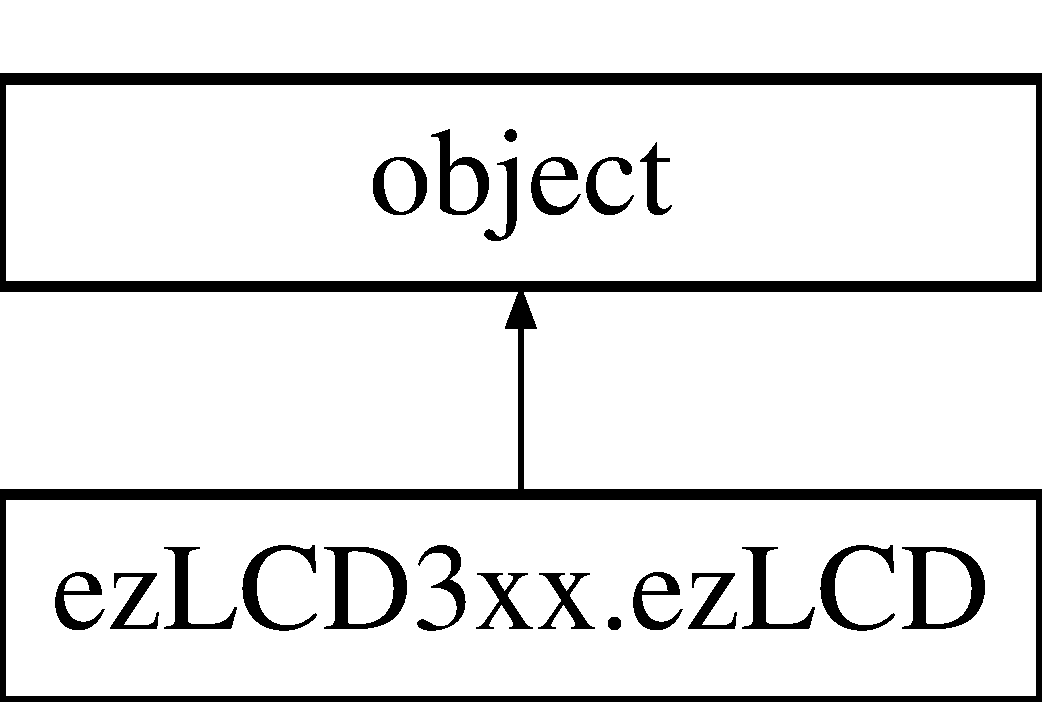
\includegraphics[height=2.000000cm]{d0/dc0/classez_l_c_d3xx_1_1ez_l_c_d}
\end{center}
\end{figure}


The documentation for this class was generated from the following file\-:\begin{DoxyCompactItemize}
\item 
C\-:/\-Users/\-Segler/\-Documents/\-Git\-Hub/ez\-L\-C\-D3xx\-Python/module/ez\-L\-C\-D3xx.\-py\end{DoxyCompactItemize}

\addcontentsline{toc}{part}{Index}
\printindex
\end{document}
